\documentclass[oneside]{scrbook} %%% remove oneside option for final hard copy
\usepackage[onehalfspacing]{setspace} %%% remove this option for final copy

%%% EDITING TOOLS
%%% use this command to load only certain chapters during writing/editing process (cross-referencing with omitted chapters will still work):
\includeonly{background}

%%% FORMATTING
%%%Probably best to put formatting commands in a separate file. Consider changing: fonts, margins (must be at least 4cm at left and 1.5cm around edges), header/footer, references/citations, algorithms, captions, paragraph indents, chapter/equation numbering, ...
\usepackage{epigraph}
\setlength{\epigraphwidth}{0.6\linewidth}
\renewcommand{\textflush}{flushright} %%% default is flushleft, not sure which looks better

%%% BIBLIOGRAPHY
\usepackage[style=authoryear, sorting=nyt, backend=biber]{biblatex} %%% use \cite, \textcite and \parencite commands in text
\addbibresource{../latex/smc.bib}

%%% MATHS PACKAGES

%%% USER-DEFINED MACROS


\begin{document}

\begin{titlepage}
\centering
\vspace*{5cm}
\begin{LARGE}\bfseries
Resampling and genealogies in sequential Monte Carlo algorithms\par \end{LARGE} 
\vspace{1.5cm} 
\begin{Large}\bfseries
Susanna Elizabeth Brown\par
\end{Large}
\vspace{3cm}
\begin{large}
A thesis submitted for the degree of\\Doctor of Philosophy in Statistics \par
\vspace{1.5cm}
University of Warwick, Department of Statistics \par
\vspace{1.5cm}
Janurary 2021 %%% update submission date (month year)
\end{large}
\end{titlepage}


\frontmatter

\tableofcontents
\listoffigures
\listoftables
\chapter{Acknowledgements}
I would like to thank... %%% supervisors, funding body, people who helped me with research, other people who supported me
\vspace*{3cm}

%%% Edit the declaration as appropriate:
%%% Add a section title above the declaration?

This thesis is submitted to the University of Warwick in support of my application for the degree of Doctor of Philosophy. It has been composed by myself and has not been submitted in any previous application for any degree %%% (if parts previously used add:) apart from the background material in sections XXX which was previously submitted for YYY degree.
\\[5pt]
The work presented (including data generated and data analysis) was carried out by the author except in the cases outlined below:
%%% List of data provided and/or analysis carried out by collaborators.
\\[5pt]
Parts of this thesis have been published by the author:
%%% List of publications including submitted papers.

\chapter{Abstract} %%% remove the "Abstract" title?

%%% The abstract must be no more than 300 words and may be single-spaced to ensure it fits on one page.

%%% A list of acronyms must be placed either here or at the end of the thesis, and its location indicated in the ToC.


\mainmatter

%%% Note: maximum word count is 70,000 excluding equations, tables, appendices etc. This is unlikely to be restrictive.

%%% The main body will be contained in separate tex files for each chapter, which are pulled in using these commands:

\chapter{Introduction}

\epigraph{
I wonder why. I wonder why.\\
I wonder why I wonder.\\
I wonder \emph{why} I wonder why\\
I wonder why I wonder!
}
{\textsc{Richard P. Feynman}}

Since their introduction in the 1990s, sequential Monte Carlo (SMC) methods, sometimes known as particle filters, have found applications in virtually every branch of science. 
This is due to the ubiquity of the types of problems in which SMC is most powerful.
As more and more data are collected and scientific models made ever more complex, practitioners are frequently reaching for numerical methods to solve problems.
SMC is a likely candidate whenever the aim is to make inferences from sequentially-observed data.
Moreover, SMC is used as a tool to speed up other numerical methods, by artificially introducing some sequential structure, for instance: tempering to enable Monte Carlo sampling from multimodal distributions; constructing nested sequences of events to enable rare event simulation; or sequentially decreasing the tolerance level in approximate Bayesian computation.

Almost three decades of study have produced a menagerie of variations on the standard ``bootstrap'' SMC algorithm, along with a deeper understanding of their theoretical underpinnings.
Even so, the problems to which SMC is applied are inherently hard,
so there are still problems to overcome.
% --- after all, Monte Carlo is said to be a last resort for problems too hard to solve in any sensible way --- 
%so it is still lacking in some respects.
One such unresolved issue, which is the primary concern of the current work, is that of ancestral or path degeneracy, which is described in Section~\ref{sec:anc_degen}. Although this problem was noted in the original article on SMC by \textcite{gordon1993}, it still has not been adequately solved.

The current work makes no attempt to provide solutions to the problem of ancestral degeneracy. The focus is instead on analysing and quantifying it, using a combination of techniques from the SMC and population genetics literatures. 
The hope is that, equipped with more information about this phenomenon, the practitioner will be able to make better judgements about their choice of algorithm and tuning parameters, and how much trust they should put in the resulting estimates.
\\[10pt]

The bulk of the thesis is divided into four chapters. 
Chapter~\ref{ch:bg} provides the relevant background on sequential Monte Carlo and coalescent theory, and explains in more detail the relevance of genealogies to the study of SMC algorithms.
It also includes a detailed comparison of the most important ``resampling schemes'' in the SMC literature, in terms of various properties of interest. Most of the results included are well-known, but Section~\ref{sec:resampling_properties} provides a more complete summary than can be found elsewhere in the literature.

Chapter~\ref{ch:limits} sets up the framework for the asymptotic analysis of genealogies, and presents the first result (Theorem~\ref{thm:FDDconv}), a sufficient condition for convergence of finite-dimensional distributions to those of Kingman's $n$-coalescent (Section~\ref{sec:KC}). The proof of the theorem builds on a related result of \textcite{koskela2018}, which is reviewed in Section~\ref{sec:existing}.

In Chapter~\ref{ch:weakconv} it is shown that under the same sufficient conditions, the processes under consideration also converge \emph{weakly} to the $n$-coalescent (Theorem~\ref{thm:weakconv}), the first weak convergence result for SMC genealogies. This is a stronger result than that of Chapter~\ref{ch:limits}, additionally requiring tightness of the processes.

Chapter~\ref{ch:appl} consists of a series of corollaries, each of which verifies the theorem conditions for a particular class of SMC algorithms. This includes the majority of SMC algorithms commonly used by practitioners.


\chapter{Background}

\epigraph{
Anyone who considers arithmetical methods of producing random digits is, of course, in a state of sin.
}
% For, as has been pointed out several times, there is no such thing as a random number --- there are only methods to produce random numbers, and a strict arithmetic procedure of course is not such a method.
{\textsc{John von Neumann}}


\section{Sequential Monte Carlo}

\subsection{Motivation}
\draft{Being Bayesian. SSMs/HMMs. Example(s) of SSM (1D train?).}

\subsection{Inference in SSMs}
\draft{What quantities do we want to infer? Why is this generally difficult? Filtering, prediction, smoothing, likelihood/normalising constant.}

\subsection{Exact solutions}
\seb{This section needs redrafting, but all the content I wanted is here.}
\draft{What about ensemble Kalman filter?}

In the case of linear Gaussian state space models, the posterior distributions of interest are also Gaussian, with mean and covariance available analytically by way of the Kalman filter \parencite{kalman1960} and Rauch-Tung-Striebel (RTS) smoother recursions \parencite{rauch1965}. Recursions are also available for some other conjugate models: see for example \textcite{vidoni1999}.
Another analytic case occurs if the state space $\mathcal{X}$ is finite, in which case any integrals become finite sums, and the forward-backward algorithm \parencite{baum1970} yields the exact posteriors.

If the model is Gaussian but non-linear, the posterior filtering distributions can be estimated using the \emph{extended Kalman filter} (see for example \textcite{jazwinski2007}), which applies a first-order linearisation in order to make use of the Kalman filter. This method performs well on models that are ``almost linear''. The resulting predictor is only \emph{optimal} when the model is actually linear, in which case the extended Kalman filter coincides with the Kalman filter.

For models that are highly non-linear or for which gradients are not readily available, a more suitable method is the \emph{unscented Kalman filter} \parencite{wan2000}. This involves taking a representative sample (which is chosen deterministically using the \emph{unscented transformation}) to characterise the distribution at time $t$, and then propagating these points through the non-linear transition $F$ to obtain a characterisation of the distribution at time $t+1$. \seb{This is getting closer to SMC, hmm?}

In more complex models such techniques are not feasible, and we are forced to resort to Monte Carlo methods.
For state space models, Markov chain Monte Carlo methods perform woefully due to the high dimension of the parameter space and high correlation between dimensions. 
But we can exploit the sequential nature of the underlying dynamics to decompose the problem into a sequence of inferences of more manageable dimension.
This is the motivation behind sequential Monte Carlo (SMC) methods.


\subsection{Feynman-Kac models}
\draft{Define a generic FK model. Show that this class includes all SSMs. Example of non-SSM that is FK?}

\subsection{Sequential Monte Carlo for Feynman-Kac models}
\draft{Present generic algorithm. State the SMC estimators of the quantities of interest. Include the dependence diagram and note that the offspring counts are not independent at each time, but can be made so by conditioning on the separatrix $\mathcal{H}$.}

\vspace{10pt}
\begin{algorithm}
\DontPrintSemicolon
\KwData{$N, T, \mu, (K_t)_{t=1}^T, (g_t)_{t=0}^T$}
\lFor{$i \in \{1,\dots,N\}$}{ 
	Sample $X_0^{(i)} \sim \mu(\cdot)$
}
\lFor{$i \in \{1,\dots, N\}$}{
		$w_{0}^{(i)} \gets  \left\{{\sum_{j=1}^N g_0(X_0^{(j)})}\right\}^{-1}{g_0(X_0^{(i)})} $ 
	}
\For{$t \in \{0,\dots, T-1\}$}{
	Sample $a_t^{(1:N)} \sim $ \textsc{resample}$(\{1,\dots ,N\}, w_t^{(1:N)}$)\;
	\lFor{$i \in \{1,\dots,N\}$}{
		Sample $X_{t+1}^{(i)} \sim K_{t+1}(X_t^{(a_t^{(i)})}, \cdot)$
	}
	\lFor{$i \in \{1,\dots, N\}$}{	
		$w_{t+1}^{(i)} \gets \Big\{ {\sum_{j=1}^Ng_{t+1}(X_t^{(a_t^{(j)})},X_{t+1}^{(j)}) }\Big\}^{-1} g_{t+1}(X_t^{(a_t^{(i)})},X_{t+1}^{(i)}) $
	}
}
\caption{Sequential Monte Carlo}\label{alg:SMC}
\end{algorithm}
\vspace{10pt}

Figure \ref{fig:cond_indep_graph} shows part of the conditional dependence graph implied by Algorithm \ref{alg:SMC}. Our aim is to find a $\sigma$-algebra $\mathcal{H}_t$ at each time $t$ that separates the ancestral process (encoded by $a_t^{(1:N)}$) from the filtration $\mathcal{F}_{t-1}$. That is, $a_t^{(1:N)}$ is conditionally independent of $\mathcal{F}_{t-1}$ given $\mathcal{H}_t$.
By a D-separation argument \parencite[see][]{verma1988}, the nodes highlighted in grey suffice as the generator of $\mathcal{H}_t$. That is, for each $t$, we take
\begin{equation*}
\mathcal{H}_t = \sigma(X_{t-1}^{(1:N)}, X_t^{(1:N)}, w_{t-1}^{(1:N)}, w_t^{(1:N)} ).
\end{equation*}
Notice that $\nu_t^{(1:N)}$ can be expressed as a function of $a_t^{(1:N)}$, and as such carries less information.
\begin{figure}[h]
\centering
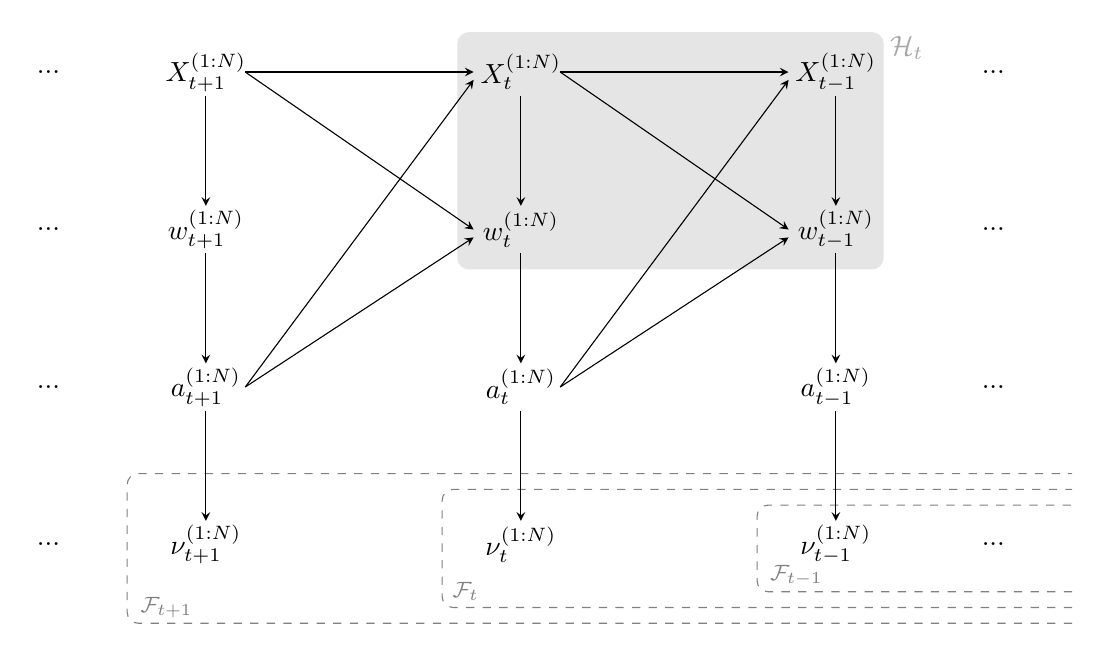
\begin{tikzpicture}[>=stealth]
% separatrix
\filldraw[gray!20, rounded corners] (3.2,0.5)--(8.6,0.5)--(8.6,-2.5)--(3.2,-2.5)--cycle;
\node[gray!70] at (8.9,0.3) {$\mathcal{H}_t$};
% left dots
\node at (-2,0) {...};
\node at (-2,-2) {...};
\node at (-2,-4) {...};
\node at (-2,-6) {...};
% labels (t+1)
\node at (0,0) {$X_{t+1}^{(1:N)}$};
\node at (0,-2) {$w_{t+1}^{(1:N)}$};
\node at (0,-4) {$a_{t+1}^{(1:N)}$};
\node at (0,-6) {$\nu_{t+1}^{(1:N)}$};
% labels t
\node at (4,0) {$X_{t}^{(1:N)}$};
\node at (4,-2) {$w_{t}^{(1:N)}$};
\node at (4,-4) {$a_{t}^{(1:N)}$};
\node at (4,-6) {$\nu_{t}^{(1:N)}$};
% labels (t-1)
\node at (8,0) {$X_{t-1}^{(1:N)}$};
\node at (8,-2) {$w_{t-1}^{(1:N)}$};
\node at (8,-4) {$a_{t-1}^{(1:N)}$};
\node at (8,-6) {$\nu_{t-1}^{(1:N)}$};
% right dots
\node at (10,0) {...};
\node at (10,-2) {...};
\node at (10,-4) {...};
\node at (10,-6) {...};
%filtrations
\draw [rounded corners, dashed, gray] (11,-6.6)--(7,-6.6)--(7,-5.5)--(11,-5.5);
\draw [rounded corners, dashed, gray] (11,-6.8)--(3,-6.8)--(3,-5.3)--(11,-5.3);
\draw [rounded corners, dashed, gray] (11,-7)--(-1,-7)--(-1,-5.1)--(11,-5.1);
% filtration labels
\node[gray] at (7.5,-6.4) {\footnotesize{$\mathcal{F}_{t-1}$}};
\node[gray] at (3.3,-6.6) {\footnotesize{$\mathcal{F}_{t}$}};
\node[gray] at (-0.5,-6.8) {\footnotesize{$\mathcal{F}_{t+1}$}};
% arrows (t+1) -> t
\draw[->] (0.5,0)--(3.4,0);
\draw[->] (0.5,0)--(3.4,-2);
\draw[->] (0.5,-4)--(3.4,-2.1);
\draw[->] (0.5,-4)--(3.4,-0.1);
% arrows t -> (t-1)
\draw[->] (4.5,0)--(7.4,0);
\draw[->] (4.5,0)--(7.4,-2);
\draw[->] (4.5,-4)--(7.4,-2.1);
\draw[->] (4.5,-4)--(7.4,-0.1);
% vertical arrows (t+1)
\draw[->] (0,-0.3)--(0,-1.7);
\draw[->] (0,-2.3)--(0,-3.7);
\draw[->] (0,-4.3)--(0,-5.7);
% vertical arrows t
\draw[->] (4,-0.3)--(4,-1.7);
\draw[->] (4,-2.3)--(4,-3.7);
\draw[->] (4,-4.3)--(4,-5.7);
% vertical arrows (t-1)
\draw[->] (8,-0.3)--(8,-1.7);
\draw[->] (8,-2.3)--(8,-3.7);
\draw[->] (8,-4.3)--(8,-5.7);
\end{tikzpicture}
\caption[Conditional dependence structure of SMC algorithm]{Part of the conditional dependence graph implied by Algorithm \ref{alg:SMC}. The direction of time is from left to right. The reverse-time filtration is indicated by the dashed areas. The nodes highlighted in grey generate the separatrix $\mathcal{H}_t$ between $a_t^{(1:N)}$ and $\mathcal{F}_{t-1}$.\seb{Use the same shades of grey here as elsewhere}}
\label{fig:cond_indep_graph}
\end{figure}


\subsection{Theoretical justification}
\draft{How come SMC works? Convergence results (briefly!) e.g. Lp bounds, CLT, stability.}


\section{Coalescent theory}

\subsection{Kingman's coalescent}
The Kingman coalescent \parencite{kingman1982gene, kingman1982coal, kingman1982exch} is a continuous-time Markov process on the space of partitions of $\mathbb{N}$. For our purposes we need only consider its restriction to $\{1,\dots,n\}$, termed the $n$-coalescent (defined below), since we only ever consider finite samples from a population. 
However, an excellent probabilistic introduction to the Kingman coalescent from the point-of-view of exchangeable random partitions can be found in \textcite[Chapters 1--2]{berestycki2009}. \seb{or \textcite{wakeley2009} ? or \textcite{durrett2008} ?}
\begin{defn}
\label{def:kingman}
The \emph{$n$-coalescent} is the homogeneous continuous-time Markov process on the set of partitions of $\{1,\dots,n\}$ with infinitesimal generator $Q$ having entries
\begin{equation}\label{eq:KCgenerator}
q_{\xi,\eta} = \begin{cases}
1 & \xi \prec \eta\\
-|\xi|(|\xi|-1)/2 & \xi=\eta \\
0 & \text{otherwise}
\end{cases}
\end{equation}
where $\xi$ and $\eta$ are partitions of $\{1,...,n\}$, $|\xi|$ denotes the number of blocks in $\xi$, and $\xi \prec \eta$ means that $\eta$ is obtained from $\xi$ by merging exactly one pair of blocks.
\end{defn}

\begin{figure}
\centering
\includegraphics[width=0.6\textwidth, trim={2.8cm 3cm 1.5cm 2cm}, clip]{plots/ncoalescent.pdf}
\caption[The $n$-coalescent]{A realisation of the $n$-coalescent with $n=50$.}
\end{figure}

A particularly attractive feature of the $n$-coalescent is its tractability; its distribution and those of many statistics of interest are available in closed form (Section \ref{sec:KCproperties}).
It turns out also to be extremely useful as a limiting distribution in population genetics, including the genealogies of a wide range of population models in its domain of attraction (Section \ref{sec:popgenmodels}).


\subsection{Properties}\label{sec:KCproperties}
The simplicity of $Q$ allows various properties of the $n$-coalescent to be studied analytically. \seb{Refer to more exhaustive studies of the properties in the literature, e.g.\ \textcite[Section 1.2]{durrett2008}.}
Starting with $n$ blocks, exactly $n-1$ coalescences are required to reach the absorbing state where all blocks have coalesced, known in the population genetics literature as the \emph{most recent common ancestor} (MRCA).

\begin{figure}[ht]
\centering
\begin{tikzpicture}
% horizontal lines
\draw[dotted, gray] (-0.5,-1)--(6,-1);
\draw[dotted, gray] (-0.5,-0.2)--(6,-0.2);
\draw[dotted, gray] (-0.5,0.5)--(6,0.5);
\draw[dotted, gray] (-0.5,1.3)--(6,1.3);
\draw[dotted, gray] (-0.5,3.3)--(6,3.3);

% tree
\draw[thick] (0,-1)--(0,-0.2);
\draw[thick] (1,-1)--(1,-0.2);
\draw[thick] (0,-0.2)--(1,-0.2);
\draw[thick] (0.5,-0.2)--(0.5,1.3);
\draw[thick] (2,-1)--(2,1.3);
\draw[thick] (0.5,1.3)--(2,1.3);
\draw[thick] (3,-1)--(3,0.5);
\draw[thick] (4,-1)--(4,0.5);
\draw[thick] (3,0.5)--(4,0.5);
\draw[thick] (1.25,1.3)--(1.25,3.3);
\draw[thick] (3.5,0.5)--(3.5,3.3);
\draw[thick] (1.25,3.3)--(3.5,3.3);

% interval arrows
\draw[<->] (5,-1)--(5,-0.2);
\draw[<->] (5,-0.2)--(5,0.5);
\draw[<->] (5,0.5)--(5,1.3);
\draw[<->] (5,1.3)--(5,3.3);

% small t's
\node at (5.2, -0.6) {\footnotesize{$t_5$}};
\node at (5.2, 0.15) {\footnotesize{$t_4$}};
\node at (5.2, 0.9) {\footnotesize{$t_3$}};
\node at (5.2, 2.3) {\footnotesize{$t_2$}};

% capital T's
\node[anchor=west] at (6, -1) {\footnotesize{$T_5 = 0$}};
\node[anchor=west] at (6, -0.2) {\footnotesize{$T_4$}};
\node[anchor=west] at (6, 0.5) {\footnotesize{$T_3$}};
\node[anchor=west] at (6, 1.3) {\footnotesize{$T_2$}};
\node[anchor=west] at (6, 3.3) {\footnotesize{$T_1 = T_{MRCA}$}};
\end{tikzpicture}
\caption{Diagram illustrating the definitions of $t_i$, $T_i$ in the $n$-coalescent.}
\label{fig:KC_timedefns}
\end{figure}

Denote by $t_2, t_3 \dots, t_n$ the waiting times between coalescent events, where $t_i$ is the amount of time for which the coalescent has exactly $i$ distinct lineages (see Figure~\ref{fig:KC_timedefns}).
A consequence of Definition~\ref{def:kingman} is that these waiting times are independent and have distributions
\begin{equation}
t_i \sim \Exp\left( \binom{i}{2} \right) .
\end{equation}
The partial sum $T_k := \sum_{i=k+1}^n t_i$ gives the total time up to the $(n-k)^{th}$ coalescence event, i.e.\ the first time at which there are only $k$ lineages remaining out of the initial $n$ (see Figure~\ref{fig:KC_timedefns}).
The partial sums, being sums of independent Exponential random variables, have HyperExponential distributions.


\subsubsection{Time to MRCA}
Of particular interest is the tree height or time to the most recent common ancestor, $T_{MRCA} := T_1$.
With some algebra we find, for instance,
\begin{equation}
\E[ T_{MRCA} ] 
= \sum_{i=2}^{n} \E[t_i]
= \sum_{i=2}^n \frac{2}{i(i-1)}
= 2 \sum_{i=2}^n \left\{ \frac{1}{i-1} - \frac{1}{i} \right\}
= 2 \left( 1 - \frac{1}{n} \right)
\end{equation}
and
\begin{equation}
\V[ T_{MRCA} ] 
= \sum_{i=2}^n \V[t_i]
= \sum_{i=2}^n \left( \frac{2}{i(i-1)} \right)^2 .
\end{equation}
The expected tree height converges to 2 as $n\to\infty$, and the variance converges to $4(\pi^2 - 9)/3 \simeq 1.16$.
The somewhat surprising fact that the tree height does not diverge with $n$ is a result of the very high rate of coalescence close to the bottom of the tree. This rate is large enough that the full Kingman coalescent (on $\mathbb{N}$) \emph{comes down from infinity}, that is, despite starting with infinitely many blocks, after any positive amount of time these have coalesced into finitely many blocks.
\seb{Plot mean with sd-ribbon over $n$ for an illustration? SD ribbon isn't the right thing; since we apparently know the actual distribution, plot a high density interval of that. (also for $L$)}


\subsubsection{Total branch length}
Another quantity of interest is the total branch length,
$ L := \sum_{i=2}^n i t_i $.
For instance
\begin{equation}
\E[ L ] 
= \sum_{i=2}^n i \E[ t_i ]
= \sum_{i=2}^n \frac{2}{i-1}
= \sum_{i=1}^{n-1} \frac{2}{i} %,
\simeq 2 \ln(n-1) 
\end{equation}
%a harmonic series, 
and
\begin{equation}
\V[ L ] 
= \sum_{i=2}^n i^2 \V[ t_i ]
= \sum_{i=2}^n \frac{4}{(i-1)^2}
= \sum_{i=1}^{n-1} \frac{4}{i^2} .
\end{equation}
Note that although the mean total branch length diverges with $n$, the variance converges to a constant, $4\pi /6 \simeq 6.6$.


\subsubsection{Probability that sample MRCA equals population MRCA}
One other interesting quantity is the probability that the MRCA of $k$ random lineages coincides with the population MRCA \parencite[e.g.][Theorem 1.7]{durrett2008}.
Denote by $S_k$ the relevant event: that a random sample of $k$ lineages has the same as the MRCA as the population.
Consider the two subtrees produced by cutting the tree just below the population MRCA. The sample of $k$ lineages coalesces before the population MRCA if and only if all $k$ sampled leaves lie in just one of these two subtrees.
A basic consequence of the exchangeability of the $n$-coalescent is that, in the limit $N\to\infty$, the proportion of leaves in the left subtree is uniformly distributed on $[0,1]$.
Calling this proportion $X$, we have
\begin{equation*}
\Prob [ S_k^c \mid X=x]
= x^k + (1-x)^k
\end{equation*}
Integrating against the distribution of $X$, the probability of interest is
\begin{equation*}
\Prob[ S_k ]
= 1- \int_0^1 [ x^k + (1-x)^k ] dx
= \frac{k-1}{k+1}
\end{equation*}
as required.

The above is based on properties of the full Kingman coalescent, but similar results are available for the $n$-coalescent.
Consider now a subsample of size $k$ among $n$ lineages that follow the $n$-coalescent.
Denote by $S_{k,n}$ the event that these $k$ lineages have the same MRCA as all $n$ lineages.
This probability of this event is calculated in \textcite[Example 1]{saunders1984} and again in \textcite[Equation (3)]{spouge2014}, in both cases arising as a special case of more general results. A direct proof is given below.

Let $X$ be the number of leaves in the left subtree. So $X \in \{1,\dots,n-1\} $ and, like before, a consequence of exchangeability is that $X$ is uniformly distributed on that set.
Now that the total number of branches is finite, we have to count more carefully. Conditional on $X$ we have
\begin{equation*}
\Prob [S_{k,n}^c \mid X=x]
= \left[ \binom{x}{k} + \binom{n-x}{k} \right] \binom{n}{k}^{-1} .
\end{equation*}
Integrating against the distribution of $X$ gives
\begin{align*}
\Prob[ S_{k,n} ]
&= 1 - \frac{1}{n-1} \binom{n}{k}^{-1} \, \sum_{x=1}^{n-1} 
        \left[ \binom{x}{k} + \binom{n-x}{k} \right] \\
&= 1 - \frac{1}{n-1} \binom{n}{k}^{-1} 
        \left[ \binom{n}{k+1} + \binom{n}{k+1} \right] \\
&= \frac{k-1}{k+1} \frac{n+1}{n-1}
\end{align*}
using binomial identities and some algebra.
As $n\to\infty$ this agrees with the population-level result above.



\subsection{Models in population genetics}\label{sec:popgenmodels}
The Kingman coalescent is the limiting coalescent process (in the large population limit) for a surprisingly wide range of population models. Some important examples of models in Kingman's ``domain of attraction'' are introduced in this section.
Common to all of these models are the following assumptions:
\begin{itemize}
\item The population has constant size $N$
\item Reproduction happens in discrete generations
\item The offspring distributions are identical at each generation, and independent between generations
\item These models are all \emph{neutral}, i.e.\ the offspring distribution is exchangeable.
\end{itemize}
As before \seb{section/eq ref?}, we define offspring counts in terms of parental indices as $\nu_j := |\{ i: a_i = j\}|$.
Under the assumption of neutrality, it is sufficient to consider only the offspring counts, rather than the parental indices (which generally carry more information).
\seb{Crucially, in the neutral case, offspring counts carry all the information about the distribution of the genealogy that is contained in the parental indices.}
From a biological perspective, neutrality encodes the absence of natural selection, i.e.\ no individual in the population is ``fitter'' than another.

\subsubsection{Wright-Fisher model}
The neutral Wright-Fisher model \parencite{fisher1923, fisher1930, wright1931} is one of the most studied models in population genetics.
At each time step the existing generation dies and is replaced by $N$ offspring. The offspring descend from parents $(a_1, \dots, a_N)$ which are selected according to
\begin{equation*}
a_i \overset{iid}{\sim} \Cat(\{1, \dots, N\}, (1/N, \dots, 1/N)).
\end{equation*}
The joint distribution of the offspring counts is therefore
\begin{equation*}
(v_1,\dots, v_N) \sim \Mn(N, (1/N, \dots, 1/N)).
\end{equation*}
Since the Multinomial distribution is exchangeable, this model is neutral.
There are several non-neutral variants of the Wright-Fisher model \seb{citations?}, but they are typically much less tractable than the neutral one.

Kingman showed in his original papers introducing the Kingman coalescent \parencite{kingman1982gene} that, when time is scaled by a factor of $N$, genealogies of the neutral Wright-Fisher model converge to the Kingman coalescent as $N\to\infty$.

\subsubsection{Cannings model}
The neutral Cannings model \parencite{cannings1974, cannings1975} is a more general construction which encompasses the neutral Wright-Fisher model as a special case.

In the Cannings model, the particular offspring distribution is not specified; we only require that it is exchangeable, i.i.d.\ between generations, and preserves the population size. In particular, the probability of observing offspring counts $(v_1, \dots, v_N)$ must be invariant under permutations of this vector.

Genealogies of the neutral Cannings model also converge to the Kingman coalescent, under some conditions and a suitable time-scaling \seb{which is what?}, as $N\to\infty$ \parencite[see for example][Section 2.2]{etheridge2011}. \seb{original reference for this? is not any Kingman 1982 papers, and certainly not Cannings 1974/5 which predates KC}

\subsubsection{Moran model}
The neutral Moran model \parencite{moran1958}, while perhaps less biologically relevant, is mathematically appealing because its simple dynamics make it particularly tractable.

At each time step, an ordered pair of individuals is selected uniformly at random. The first individual in this pair dies (i.e.\ leaves no offspring in the next generation), while the other reproduces (leaving two offspring). All of the other individuals leave exactly one offspring.
%Usually the model is thought of as having ``overlapping generations'': the individuals having one offspring are considered to be not reproducing but rather surviving to appear again in the next generation.
%However, one can equally think of it as having non-overlapping generations and a low variance reproduction mechanism.
This is another special case of the neutral Cannings model, where the offspring distribution is now uniform over all permutations of $(0,2,1,1,\dots,1)$.
Therefore we know that under a suitable time-scaling, its genealogies converge to the Kingman coalescent. The time scale in this case is $N^2$, because reproduction happens at a rate $N$ times \seb{or is it technically N-1 times?} lower than in the Wright-Fisher model. \seb{also cite a Moran-specific convergence result: not sure where (it isn't in Kingman 1982* or in Moran 1958 which predates KC)}


\subsection{Particle populations}
Much of the population genetics framework transfers readily to the case of SMC. The population is now a population of particles, with each iteration of the SMC algorithm corresponding to a generation, and resampling playing the part of reproduction.
In fact, SMC ``populations'' are in some ways more suited to these population models than actual populations of organisms.
The assumptions that the population has constant size $N$ and that reproduction occurs only at discrete generations are satisfied by construction.
However, we cannot assume independence between generations: as seen in Figure~\ref{fig:cond_indep_graph}, the offspring counts at subsequent generations are not independent without some conditioning. In fact, after marginalising out the information about the positions of the particles, the genealogical process is not even Markovian.
Nor is our model neutral: the resampling distribution depends on the weight of each particle (the weight plays the role of fitness in a non-neutral population model).

\section{Sequential Monte Carlo genealogies}

\subsection{From particles to genealogies}
\draft{How does the SMC algorithm induce a genealogy? (resampling = parent-child relationship).}

\subsection{Performance}
\draft{How do genealogies affect performance? Variance (and variance estimation?), storage cost. Ancestral degeneracy.}

\subsection{Mitigating ancestral degeneracy}
\draft{Low-variance resampling (save details for next section). Adaptive resampling: idea of balancing weight/ancestral degeneracy; rule of thumb for implementing it; when is it effective or not?; necessary changes to our generic SMC algorithm (calculation of weights in particular). Backward sampling: when is it possible to do this?}

\subsection{Asymptotics}
\draft{Why are large population asymptotics useful? Existing results (path storage, KJJS).}



\section{Resampling}

\subsection{Definition}
As we have seen, resampling is necessary within SMC to ``reset'' the weights in order to prevent weight degeneracy.
The basic role of a resampling scheme is to map the continuous weights to discrete offspring counts, in some ``sensible'' way (Definition~\ref{defn:resampling}).
There are other considerations when choosing between the many possible resampling schemes; some of these are explored in Section~\ref{sec:goodresampling}, and some popular choices of resampling scheme are described in Section~\ref{sec:examples_resamplingschemes}.

\begin{defn}\label{defn:resampling}
For our purposes, a valid resampling scheme is a stochastic function mapping weights 
$w_t^{(1:N)} \in \mathcal{S}_{N-1}$ 
to offspring counts 
$\nu_t^{(1:N)} \in \{0,\dots,N\}^N $
that satisfies the following properties:
\begin{enumerate}
\item\label{item:resampling_property1} the population size is conserved:
$ \sum_{i=1}^N \nu_t^{(i)} =N $ for all $N$
\item\label{item:resampling_property2} the weights are uniform after resampling:
$w_{t+}^{(i)} = 1/N$ for all $i$
\item\label{item:resampling_property3} the resampling is unbiased:
$ \E[ \nu_t^{(i)} \mid w_t^{(i)} ] = N w_t^{(i)} $ for all $i$.
\end{enumerate}
\end{defn}
It is possible to design resampling schemes that violate these properties.
For example, a scheme of \textcite{liu1998} uses the square roots of the weights for resampling, then corrects by setting non-uniform weights after resampling (violating conditions \ref{item:resampling_property2} and \ref{item:resampling_property3}).
Resampling different numbers of particles in different iterations (violating condition \ref{item:resampling_property1}) is of course possible, but we typically have a fixed limit on computational resources, in which case it makes sense to simulate the maximum feasible number of particles $N$ at every iteration.
Deterministic resampling schemes (which cannot generally be unbiased, violating condition \ref{item:resampling_property3}) have been used by some authors. These include schemes based on optimal transport \parencite{reich2013, myers2021, corenflos2021} and the importance support points resampling of \textcite{huang2020}.
However, the majority of resampling schemes in the literature fit within Definition~\ref{defn:resampling}, and it is not typically advantageous to violate the properties \ref{item:resampling_property1}--\ref{item:resampling_property3}.



\subsection{What makes a good resampling scheme?}\label{sec:goodresampling}
\draft{Low-variance: variance of what? Different criteria/ definitions of optimality. Negative association. Link back to adaptive resampling: interaction between adaptive and low-variance resampling.}




\subsection{Examples}\label{sec:examples_resamplingschemes}
\draft{Tour of the key resampling schemes (multinomial, residual-*, stratified, systematic, and the worst possible scheme). Comparison of properties of these, existing results comparing schemes. Implementation considerations. Theoretical justification (or lack of). Mention computational complexity.}\\
\seb{This whole section was dumped from elsewhere and needs redrafting.}

 
\subsubsection{Multinomial resampling}
Multinomial resampling \parencite{gordon1993,efron1994} is one of the simplest resampling schemes.
The parental indices are chosen independently from $\{1, \dots, N\}$, each with probability given by the weight of the corresponding particle $w_t^{(i)}$. 
That is, 
\begin{equation*}
a_t^{(1:N)} \sim \Cat( \{1,\dots, N\}, w_t^{(1:N)} ) .
\end{equation*}
This implies the joint distribution of the offspring counts is 
\begin{equation*}
\nu_t^{(1:N)} \eqdist \operatorname{Multinomial}(N, w_t^{(1:N)} ) .
\end{equation*}
Note that in this case the parental indices are chosen independently, but the resulting offspring counts are negatively correlated.

A simple way to sample the parental indices is by inversion sampling: divide the unit interval into $N$ disjoint subintervals each of which will correspond to a certain index $i$ and has length equal to the weight $w_t^{(i)}$; then draw $N$ samples $U_i \sim \Unif(0,1)$ and classify them according to which of these subintervals they fall in.
Explicitly, the parental index assigned to child $i$ is the index $a_i$ satisfying
\begin{equation}\label{eq:syst_strat_resampling}
\sum_{j=1}^{a_i -1} w_t^{(j)} \leq U_i \leq \sum_{j=1}^{a_i} w_t^{(j)}
\end{equation}
This is illustrated in Figure \ref{fig:resampling_mn}. 
Note that there exist more efficient methods to sample from a Multinomial distribution, so the inversion method may not be used in practice.

\subsubsection{Residual resampling}
Residual resampling is described in \textcite{liu1998} and also in \textcite{whitley1994} where it is called ``remainder stochastic sampling''.

Each particle $X_{t}^{(i)}$ is deterministically assigned $\lfloor N w_t^{(i)} \rfloor$ offspring, and the remaining $R := N- \sum_{i=1}^N \lfloor N w_{t}^{(i)} \rfloor$ offspring are assigned multinomially in proportion to the unaccounted-for weight. 
This yields a vector of offspring counts
\begin{equation*}
\nu_t^{(1:N)} \eqdist \lfloor N w_t^{(1:N)} \rfloor +  \operatorname{Multinomial}(R, (N w_t^{(1:N)} - \lfloor N w_t^{(1:N)}\rfloor)/R) .
\end{equation*}
The deterministic part ensures that every particle with weight $>1/N$ is guaranteed to survive. This is a desirable property as it prevents the random loss of high-weighted particles.

\subsubsection{Stratified resampling}
Stratified resampling is introduced in \cite{kitagawa1996}.

The scheme proceeds like Multinomial resampling, except that the Uniform samples that are fed in to do the Categorical sampling are produced in a different way.
Instead of sampling $N$ independent numbers from $\operatorname{U}(0,1)$, one number is sampled uniformly from each subinterval of length $1/N$. 
That is, 
\begin{equation*}
U_i \sim \Unif \left(\frac{i-1}{N}, \frac{i}{N} \right) .
\end{equation*}
The parents are then assigned as in \eqref{eq:syst_strat_resampling}.
(Of course this means that the offspring distribution is no longer Multinomial, since parental indices are not chosen independently.)
This scheme ensures that the samples are ``well spread out'', again reducing the probability of randomly losing high-weighted particles.
The method is illustrated in Figure \ref{fig:resampling_stratified}.

\subsubsection{Systematic resampling}
Systematic resampling is described in \textcite{carpenter1999} and also in \textcite{whitley1994} where it is called ``stochastic universal sampling''.

Like stratified resampling, it constitutes a change to the random number generator for sampling from the Categorical distriubtion. 
In this scheme, only one Uniform sample is drawn, $U \sim \operatorname{U}(0,1/N)$, and the other $N-1$ samples are generated deterministically by setting
\begin{equation*}
U_i = U + \frac{i-1}{N}
\end{equation*}
for each $i \in \{1, \dots, N\}$.
The parental indices are again selected according to \eqref{eq:syst_strat_resampling}. 
The method is illustrated in Figure \ref{fig:resampling_systematic}.
This scheme again ensures the random numbers are ``well spread out'', even more so than with stratified resampling.

Systematic resampling is often preferred among practitioners because it is extremely easy to implement and also computationally efficient, requiring only one random number to be generated.

However, this scheme is known to exhibit pathological behaviour in some cases due to its dependence on the ordering of the subintervals \parencite{douc2005}. Such behaviour can be avoided by randomly permuting the intervals before sampling, and this is the recommended practice. 

\begin{figure}
\centering
\subfloat[Multinomial resampling]{
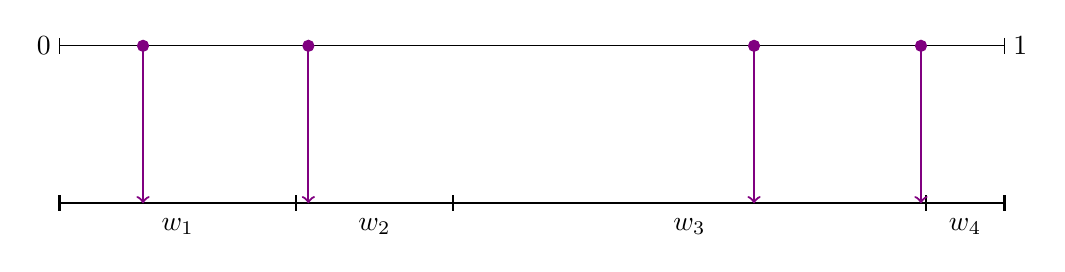
\begin{tikzpicture}
%parallel lines
\draw[thick] (0,0) -- (12,0);
\draw (0,2) -- (12,2);
% tick marks at ends
\draw[thick] (0,0.1) --(0,-0.1);
\draw[thick] (12,0.1) --(12,-0.1);
\draw (0,2.1) --(0,1.9);
\draw (12,2.1) --(12,1.9);
% tick marks indicating weights
\draw[thick] (3,0.1) --(3,-0.1);
\draw[thick] (5,0.1) --(5,-0.1);
\draw[thick] (11,0.1) --(11,-0.1);
% weight labels
\node at (1.5,-0.3) {$w_1$};
\node at (4,-0.3) {$w_2$};
\node at (8,-0.3) {$w_3$};
\node at (11.5,-0.3) {$w_4$};
% endpoint labels
\node at (-0.2,2) {$0$};
\node at (12.2,2) {$1$};
% uniform points
\filldraw[violet] (10.94,2) circle (2pt);
\filldraw[violet] (1.06,2) circle (2pt);
\filldraw[violet] (8.82,2) circle (2pt);
\filldraw[violet] (3.16,2) circle (2pt);
% arrows from random points
\draw[thick, violet, ->] (10.94,2) -- (10.94,0);
\draw[thick, violet, ->] (1.06,2) -- (1.06,0);
\draw[thick, violet, ->] (8.82,2) -- (8.82,0);
\draw[thick, violet, ->] (3.16,2) -- (3.16,0);
\end{tikzpicture}
\label{fig:resampling_mn}
}\\
\subfloat[Stratified resampling]{
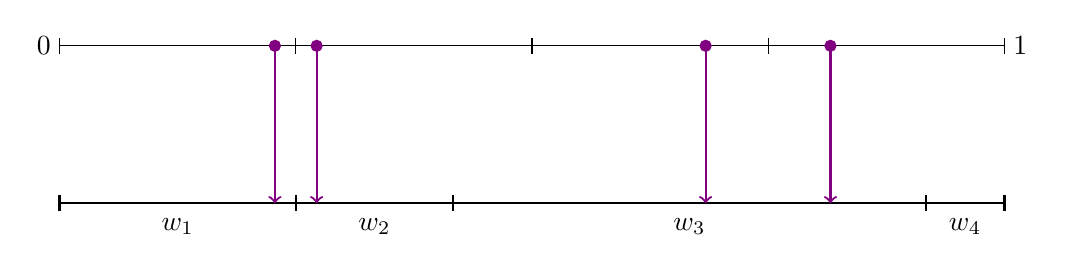
\begin{tikzpicture}
%parallel lines
\draw[thick] (0,0) -- (12,0);
\draw (0,2) -- (12,2);
% tick marks at ends
\draw[thick] (0,0.1) --(0,-0.1);
\draw[thick] (12,0.1) --(12,-0.1);
\draw (0,2.1) --(0,1.9);
\draw (12,2.1) --(12,1.9);
% tick marks indicating weights
\draw[thick] (3,0.1) --(3,-0.1);
\draw[thick] (5,0.1) --(5,-0.1);
\draw[thick] (11,0.1) --(11,-0.1);
% tick marks indicating sampling intervals:
\draw (3,2.1) --(3,1.9);
\draw (6,2.1) --(6,1.9);
\draw (9,2.1) --(9,1.9);
% weight labels
\node at (1.5,-0.3) {$w_1$};
\node at (4,-0.3) {$w_2$};
\node at (8,-0.3) {$w_3$};
\node at (11.5,-0.3) {$w_4$};
% endpoint labels
\node at (-0.2,2) {$0$};
\node at (12.2,2) {$1$};
% stratified points
\filldraw[violet] (2.735,2) circle (2pt);
\filldraw[violet] (3.265,2) circle (2pt);
\filldraw[violet] (8.205,2) circle (2pt);
\filldraw[violet] (9.79,2) circle (2pt);
% arrows from random points
\draw[thick, violet, ->] (2.735,2) -- (2.735,0);
\draw[thick, violet, ->] (3.265,2) -- (3.265,0);
\draw[thick, violet, ->] (8.205,2) -- (8.205,0);
\draw[thick, violet, ->] (9.79,2) -- (9.79,0);
\end{tikzpicture}
\label{fig:resampling_stratified}
}\\
\subfloat[Systematic resampling]{
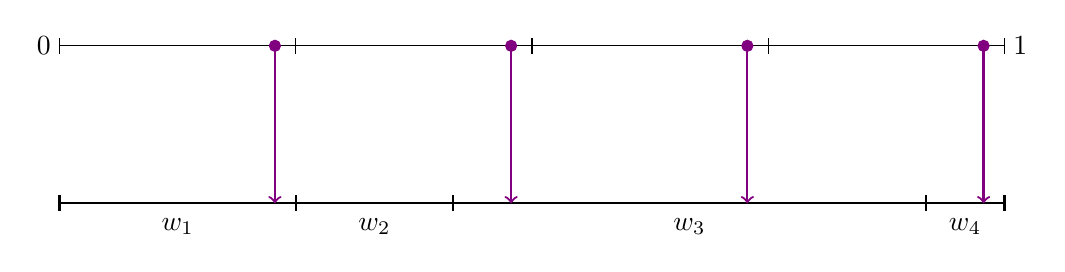
\begin{tikzpicture}
%parallel lines
\draw[thick] (0,0) -- (12,0);
\draw (0,2) -- (12,2);
% tick marks at ends
\draw[thick] (0,0.1) --(0,-0.1);
\draw[thick] (12,0.1) --(12,-0.1);
\draw (0,2.1) --(0,1.9);
\draw (12,2.1) --(12,1.9);
% tick marks indicating weights
\draw[thick] (3,0.1) --(3,-0.1);
\draw[thick] (5,0.1) --(5,-0.1);
\draw[thick] (11,0.1) --(11,-0.1);
% tick marks indicating sampling intervals:
\draw (3,2.1) --(3,1.9);
\draw (6,2.1) --(6,1.9);
\draw (9,2.1) --(9,1.9);
% weight labels
\node at (1.5,-0.3) {$w_1$};
\node at (4,-0.3) {$w_2$};
\node at (8,-0.3) {$w_3$};
\node at (11.5,-0.3) {$w_4$};
% endpoint labels
\node at (-0.2,2) {$0$};
\node at (12.2,2) {$1$};
% stratified points
\filldraw[violet] (2.735,2) circle (2pt);
\filldraw[violet] (5.735,2) circle (2pt);
\filldraw[violet] (8.735,2) circle (2pt);
\filldraw[violet] (11.735,2) circle (2pt);
% arrows from random points
\draw[thick, violet, ->] (2.735,2) -- (2.735,0);
\draw[thick, violet, ->] (5.735,2) -- (5.735,0);
\draw[thick, violet, ->] (8.735,2) -- (8.735,0);
\draw[thick, violet, ->] (11.735,2) -- (11.735,0);
\end{tikzpicture}
\label{fig:resampling_systematic}
}\\
\caption[Resampling using multinomial, stratified and systematic schemes]{Inversion sampling to obtain Multinomial offspring counts, where the Uniform variables for inversion are sampled in different ways. For this example $N=4$ and the weights are $w_{(1:4)} = \frac{1}{N}(1,\frac{2}{3},2,\frac{1}{3})$. In each case the samples to be inverted are seeded with the same $\Unif(0,1)$ samples.
\subref{fig:resampling_mn} Sample $N$  independent $\Unif(0,1)$ random variables. In this example the sampled offspring counts are $(1,1,2,0)$.
\subref{fig:resampling_stratified} The $\Unif(0,1)$ samples are transformed to Uniform draws from the intervals (0,0.25), (0.25,0.5), (0.5, 0.75), (0.75,1). In this example the sampled offspring counts are $(1,1,2,0)$.
\subref{fig:resampling_systematic} Use only the first draw and transform it to a sample from $\Unif(0,0.25)$. For the subsequent samples, add 0.25 each time to obtain a sample in each interval. In this example the sampled offspring counts are $(1,0,2,1)$.}
\end{figure}


\subsubsection{Variance}
The most straightforward choice of resampling scheme, and also the easiest to analyse, is multinomial. However, multinomial resampling is well known to be sub-optimal in terms of the resulting Monte Carlo variance, and is rarely used in practice.

\textcite{douc2005} prove that both residual resampling and stratified resampling yield lower variance estimators. 
The variance we are referring to here is the variance of Monte Carlo estimators of an arbitrary test function $f$, conditional on the past:
\begin{equation*}
\V\left[ \frac{1}{N} \sum_{i=1}^N f(X_t^{(i)}) \middle| \mathcal{F}_{t-1} \right]
\end{equation*}
The authors remark that, while the variance resulting from systematic resampling is not provably lower than that of multinomial resampling, empirical performance is comparable among residual, stratified and systematic resampling.


\subsubsection{Star discrepancy}
\draft{Something about syst vs. strat vs. mn in terms of star discrepancy (define that). See \textcite{hol2006} for inspiration.}


\subsubsection{Support of offspring numbers}
Let us consider the support of the marginal offspring distributions in each scheme, given the corresponding weight. Condition on the $i^{th}$ weight lying in the interval $w_t{(i)} \in [k/N, (k+1)/N]$, but leave the other weights unknown. By considering the best and worst cases for each scheme, we have: 
\begin{description}
\item[Multinomial:] $\nu_t^{(i)} \in \{0,\dots, N\}$
\item[Residual:] $\nu_t^{(i)} \in \{k,\dots, k+R\} \subseteq \{k,\dots, N\}$
\item[Stratified:] $\nu_t^{(i)} \in \{k-1, k, k+1, k+2\}$
\item[Systematic:] $\nu_t^{(i)} \in \{k, k+1\}$
\end{description}
We see that multinomial resampling allows the possibility of very good particles having $0$ offspring, and of very bad particles having $N$ offspring (although the probabilities associated to these events are low).
Residual resampling ensures that good particles do not die out, but still allows bad particles to possibly have many offspring.
Stratified resampling is more restrictive, although it allows the possibility of a particle with weight $>1/N$ leaving no offspring.
Systematic resampling is more restrictive still, allowing the number of offspring of each particle to vary from its expected value by no more than one.

\subsubsection{Permutation invariance}
A strange property of stratified and systematic resampling is that they are sensitive to the order in which the subintervals are placed. For example, in Figures \ref{fig:resampling_stratified} and \ref{fig:resampling_systematic} if the intervals $w_2$ and $w_4$ were swapped, the number of offspring assigned to particles 2 and 4 would be swapped in each case. 
We can also see that because $w_1$ has weight $\geq 1/N$ and is placed first, it is guaranteed at least one offspring.

This property can lead to pathological behaviour, but is easily avoided by applying a random permutation to the order of the subintervals.
\textcite{gerber2017} also propose a variation on systematic resampling that avoids this property.

\subsubsection{Degeneracy under equal weights}
Suppose we somehow end up in the situation where all the weights are equal (i.e.\ $w_t^{(i)} = 1/N$ for all $i$).
In this case, residual resampling will result in a deterministic assignment only: each particle will be assigned one offspring, and there will be no remainder left to assign randomly. This behaviour cannot be avoided, however the event that all weights are equal typically has zero measure.

Stratified and systematic resampling will have the same result: the intervals for sampling will correspond exactly to the weighted subintervals, so no matter which random numbers are sampled, exactly one will fall in each subinterval.

However, for stratified resampling, the formulation of \textcite{whitley1994} avoids this behaviour. He imagines subdivisions of a circle rather than an interval, and then ``spins the roulette wheel'' around it, which shifts the sampling intervals by a random amount and thus prevents this degeneracy.

\subsubsection{Exchangeability}
We will call a resampling scheme exchangeable if the resulting distribution of parental indices is invariant under permutations of the children. To put it another way, each child chooses its parent from the same marginal distribution.

It is clear that multinomial resampling is exchangeable since in this case the parental indices are independent and identically distributed. However it is worth noting that some efficient implementations of multinomial sampling may not preserve exchangeability in practice.

Stratified and systematic resampling are clearly not exchangeable since, for instance, child 1 is more likely to choose parent 1 than child $N$ is. However, this is merely a feature of the arbitrary ordering of the sampling steps: exchangeability can easily be reintroduced by applying a random permutation to the vector of parental indices after sampling.
The same goes for residual resampling.


\subsubsection{Computational complexity}
All of the resampling algorithms discussed above can be implemented in $O(N)$ operations.
Considering the complexity of each operation, \textcite{hol2004,hol2006} suggest that systematic resampling is fastest because it only requires one pseudo-random number generation, and multinomial resampling is slower than stratified resampling because of the transformations required. Residual resampling is hard to compare directly because a random fraction of the operations are deterministic, so the number of pseudo-random numbers required is less than $N$.
This analysis was backed up by simulation experiments.
However, the analysis of per-particle cost is sensitive to the particular implementation of each resampling scheme, the system implementation of pseudo-random number generation and arithmetic operations, and the hardware used.


\subsubsection{Optimal resampling}
\textcite{crisan1999} introduce another resampling scheme based on a branching process, which they show to be optimal in some sense. However, their algorithm is not widely used in practice because it is much more complicated to implement than alternatives like systematic resampling which perform just as well empirically, and share some of its optimality properties \parencite{bain2008}. 
 
 
 

\subsection{Stochastic rounding}
\draft{Define stochastic rounding. Resampling schemes contained by this class. General properties for this class (marginal distributions, negative association, minimum-variance).}

\begin{defn}\label{defn:stochround}
 Let $X=(X_1,\dots,X_N)$ be a $\mathbb{R}_+^N$-valued random variable. Then $Y=(Y_1,\dots,Y_N) \in \mathbb{N}^N$ is a \emph{stochastic rounding} of $X$ if each element $Y_i$ takes values
\begin{equation*}
Y_i \mid X_i =
\begin{cases}
 \lfloor X_i \rfloor & \text{with probability } 1- X_i+ \lfloor X_i \rfloor \\
  \lfloor X_i \rfloor +1 & \text{with probability } X_i- \lfloor X_i \rfloor .
\end{cases}
\end{equation*}
\end{defn}

By construction, $\E(Y_i) = X_i$ for each $i$. Taking $X$ to be $N$ times the vector of particle weights, we can therefore use stochastic rounding to construct a valid resampling scheme, under the further constraint that $Y_1 + \dots + Y_N = N$.
Several ways to enforce this constraint on the joint distribution have been proposed, including systematic resampling, residual resampling with systematic residuals, the branching system of \textcite{crisan1997}, and the Srinivasan sampling process resampling introduced in \textcite{gerber2017}.




\section{Conditional SMC}

\subsection{Particle MCMC}
\draft{Motivate particle MCMC methods.}

The idea behind particle MCMC methods is to use SMC steps within the MCMC updates in a way that improves the mixing properties of the Markov chain.
In certain models, generally those including some highly correlated sequential components, this strategy can be very effective.

The following scenario illustrates the power of particle MCMC, and is a good model to have in mind as we go on to discuss particle Gibbs and ancestor sampling.
\draft{Include the model from the start of my ancestor sampling note. Emphasise that the inference itself is not sequential; we are targeting one static posterior distribution, on a fixed time horizon.}


\subsection{Particle Gibbs algorithm}
\draft{Present particle Gibbs algorithm (for the specific model just introduced?, but note that of course the algorithm is more general). Explain why CSMC is required within particle Gibbs.}

\subsection{Ancestor sampling}
\draft{Algorithm (or required changes to generic algorithm). Relation to backward sampling. When can it be implemented? Effect on performance (when is it effective?). Maybe illustrate/motivate with some plots as in the ancestor sampling note.}

%\chapter{Limits}

%%% choose an epigraph to go here

\section{Encoding genealogies}

\subsection{The genealogical process}
\draft{Encoding as process on space of partitions $\mathcal{P}_n$. Argue that this encodes everything we need. Initial and absorbing states. Intuit with diagram(s), explain relationship between partition blocks and genealogical tree.}

\subsection{Time scale}
\draft{Introduce $c_N$, $\tau_N$, $D_N$. Contrast to pop gen literature, e.g. our $c_N$/time scale is random. Properties of these quantities: $c_N, D_N \in [0,1]$, and $D_N \leq c_N$ and $\sum_{r=1}^{\tau_N(t)} c_N \in [t, t+1]$ (or rather the version of that with general start time).}




\subsection{Transition probabilities}
\draft{Introduce $p_{\xi\eta}$. Present expression for that (or at least for $p_{\xi\xi}$), and hence the bounds on it that will be used later (keeping big-O terms explicit where possible).}

\section{An existing limit theorem}
\draft{State KJJS theorem. Discuss the conditions in detail. Give outline of proof.}

\section{A new limit theorem}
\draft{State our limit theorem. Give intuition for the new condition. Compare to KJJS: why our conditions might be considered ``weaker'' (Moran model example, and whatever else we said to our referee/in the BJJK article); our condition is easier to check (as demonstrated in later corollaries).}

\begin{theorem}\label{thm:FDDconv}
Let $\nu_t^{(1:N)}$ denote the offspring numbers in an IPS satisfying the standing assumption and such that, for any $N$ sufficiently large, $\Prob\{ \tau_N(t) = \infty \} =0$ for all finite $t$. Suppose that there exists a deterministic sequence $(b_N)_{N\geq1}$ such that ${\lim}_{N\to\infty} b_N =0$ and
\begin{equation}\label{eq:mainthmcond}
\frac{1}{(N)_3} \sum_{i = 1}^N \Et\{ (\nu_t^{(i)})_3 \}  \leq b_N \frac{1}{(N)_2} \sum_{i = 1}^N \Et\{ (\nu_t^{(i)})_2 \}
\end{equation}
for all $N$, uniformly in $t \geq 1$.
Then the rescaled genealogical process $(G_{\tau_N(t)}^{(n,N)})_{t\geq0}$ converges in the sense of finite-dimensional distributions to Kingman's $n$-coalescent as $N \to \infty$.
\end{theorem}



\subsection{Proof of theorem}
\draft{Proof that KJJS conditions are implied by ours. Modification of KJJS proof (or even write out a complete proof?) using weaker bound on $p_{\xi\xi}$ (that bound should have been stated and proved already in transition probabilities section).}
%\include{csmc}
%\chapter{Weak Convergence}

\epigraph{
At the age of twenty-one he wrote a treatise upon the Binomial Theorem, which has had a European vogue. On the strength of it he won the Mathematical Chair at one of our smaller universities, and had, to all appearances, a most brilliant career before him.
}
{\textsc{Sherlock Holmes}} %\\The Final Problem

We start by defining a suitable metric space.
Let $\mathcal{P}_n$ be the space of partitions of $\{1,\dots,n\}$.
Denote by $\mathcal{X}$ the set of all functions mapping $[0,\infty)$ to $\mathcal{P}_n$ that are right-continuous with left limits.
(Our rescaled genealogical process $(\mathcal{G}^{(n,N)}_{\tau_N(t)})_{t\geq0}$ and our encoding of the $n$-coalescent are piecewise-constant functions mapping time $t\in[0,\infty)$ to partitions, and thus live in the space $\mathcal{X}$.)
Finally, equip the space $\mathcal{P}_n$ with the zero-one metric,
\begin{equation}
\rho(\xi,\eta) 
= 1- \delta_{\xi\eta} 
:= \begin{cases}
    0 &\text{if } \xi=\eta \\
    1 &\text{otherwise}
\end{cases}
\end{equation}
for any $\xi, \eta \in \mathcal{P}_n$. 


\begin{theorem}\label{thm:weakconv}
Let $\nu_t^{(1:N)}$ denote the offspring numbers in an interacting particle system satisfying the standing assumption and such that, for any $N$ sufficiently large, for all finite $t$, $\Prob\{ \tau_N(t) = \infty \} =0$. Suppose that there exists a deterministic sequence $(b_N)_{N\geq1}$ such that ${\lim}_{N\to\infty} b_N =0$ and
\begin{equation}
\frac{1}{(N)_3} \sum_{i = 1}^N \Et\{ (\nu_t^{(i)})_3 \}  \leq b_N \frac{1}{(N)_2} \sum_{i = 1}^N \Et\{ (\nu_t^{(i)})_2 \}
\end{equation}
for all $N$, uniformly in $t \geq 1$.
Then the rescaled genealogical process $(G_{\tau_N(t)}^{(n,N)})_{t\geq0}$ converges weakly in $(\mathcal{X}, \rho)$
to Kingman's $n$-coalescent as $N \to \infty$.
\end{theorem}

\begin{proof}
The structure of the proof follows \textcite{mohle1999}, albeit with considerable technical complication due to the lack of independence between generations (non-neutrality) in our model. \seb{is this the main/only source of complication?}
Since we already have convergence of the finite-dimensional distributions (Theorem ?? \seb{refers to a previous chapter}), strengthening this to weak convergence requires relative compactness of the sequence of processes $\{ (G_{\tau_N(t)}^{(n,N)})_{t\geq0} \}_{N\in\mathbb{N}}$.

We can apply \textcite[Chapter 3, Corollary 7.4]{ethier1986}: $\mathcal{P}_n$ is finite and therefore complete and separable, and the sample paths of $(G_{\tau_N(t)}^{(n,N)})_{t\geq0}$ live in $\mathcal{X}$, so the conditions of the corollary are satisfied.
The corollary states that the sequence of processes $\{ (G_{\tau_N(t)}^{(n,N)})_{t\geq0} \}_{N\in\mathbb{N}}$ is relatively compact if and only if the following two conditions hold:
\begin{enumerate}
\item \label{item:relcomp1} For every $\varepsilon>0$, $t\geq 0$ there exists a compact set $\Gamma \subseteq \mathcal{P}_n$ such that
\begin{equation}
\liminf_{N\to\infty} \Prob[ G_{\tau_N(t)}^{(n,N)} \in \Gamma ] 
\geq 1-\varepsilon
\end{equation}
\item \label{item:relcomp2} For every $\varepsilon>0$, $t>0$ there exists $\delta>0$ such that
\begin{equation}
\liminf_{N\to\infty} \Prob[ \omega(G_{\tau_N(\cdot)}^{(n,N)}, \delta, t) < \varepsilon ] 
\geq 1-\varepsilon
\end{equation}
where 
\begin{equation}
\omega(G_{\tau_N(t)}^{(n,N)}, \delta, t) := \inf \max_{i \in [K]} 
        \sup_{u,v \in [T_{i-1}, T_i)} \rho( G_{\tau_N(u)}^{(n,N)}, G_{\tau_N(v)}^{(n,N)} )
\end{equation}
with the infimum taken over all partitions of the form $0=T_0<T_1<\cdots <T_{K-1} <t \leq T_K$ such that $\min_{i\in[K]} (T_i - T_{i-1}) > \delta$. \seb{use a different letter not $K$?}
\end{enumerate}
In our case, Condition \ref{item:relcomp1} is satisfied automatically with $\Gamma = \mathcal{P}_n$, since $\mathcal{P}_n$ is finite and hence compact. 
The intuition behind condition \ref{item:relcomp2} is that the jumps of the process must be ``well-separated''. 
In our particluar case where $\rho$ is the zero-one metric, we see that $\rho( G_{\tau_N(u)}^{(n,N)}, G_{\tau_N(v)}^{(n,N)} )$ is equal to 1 if there is a jump between times $u$ and $v$, and 0 otherwise. 
The supremum over $u,v$ then indicates whether there is a jump at any time in the interval $[T_i, T_{i-1})$. 
Similarly, the maximum over $i$ then indicates whether there is a jump within any of the intervals defined by that particular partition; this can only be equal to zero if all of the jumps occur exactly at the times $T_0, \dots, T_k$. 
The infimum over all allowed partitions, then, can only be equal to zero if no two jumps occur less than $\delta$ (unscaled) time apart, because of the restriction we placed on these partitions.

The proof is concentrated on proving Condition \ref{item:relcomp2}.
To do this, we use a coupling with another process that contains all of the jumps of the genealogical process, with the addition of some extra jumps. This process is constructed in such a way that it can be shown to satisfy Condition 2, and hence so does the genealogical process.

Define $p_t := \max_{\xi\in E} \{1 - p_{\xi\xi}(t)\} = 1 - p_{\Delta\Delta}(t)$, where $\Delta$ denotes the trivial partition of $\{1,\dots,n\}$ into singletons. For a proof that the maximum is attained at $\xi = \Delta$, see Lemma \ref{thm:maximum_pr}. 
Following \textcite{mohle1999}, we now construct the two-dimensional \seb{conditionally on $\mathcal{F}$ ?} Markov process $(Z_t, S_t)_{t \in \mathbb{N}}$ with transition probabilities
\begin{equation}
\Prob(Z_t = j , S_t = \eta \mid Z_{t-1} = i, S_{t-1} = \xi)
= \begin{cases}
1 - p_t &\quad \text{if } j=i \text{ and } \xi=\eta \\
p_{\xi\xi}(t) + p_t - 1  &\quad \text{if } j=i+1 \text{ and } \xi=\eta \\
p_{\xi\eta}(t) &\quad \text{if } j=i+1 \text{ and } \xi\neq\eta \\
0 &\quad \text{otherwise} .
\end{cases}
\end{equation}\seb{initial state?}
The construction is such that the marginal $(S_t)$ has the same distribution as the genealogical process of interest, and $(Z_t)$ has jumps at all the times $(S_t)$ does plus some extra jumps. (The definition of $p_t$ ensures that the probability in the second case is non-negative, attaining the value zero when $\xi=\Delta$.)

Denote by $0=T_0^{(N)}<T_1^{(N)}<\dots$ the jump times of the rescaled process $(Z_{\tau_N(t)})_{t\geq0}$, and by $\varpi_i^{(N)} := T_i^{(N)} - T_{i-1}^{(N)}$ the corresponding holding times.

...
\end{proof}


\section*{Bounds on sum-products}

\begin{lemma}\label{thm:sumprod1}
Fix $t>0$, $l\in\mathbb{N}$.
\begin{equation}
t^l - \left( \sum_{s=1}^{\tau_N(t)} c_N(s)^2 \right) \binom{l}{2} (t+1)^{l-2} 
\leq \sum_{s_1\neq\dots\neq s_l}^{\tau_N(t)} \prod_{j=1}^l c_N(s_j)
\leq t^l + c_N(\tau_N(t)) (t+1)^l .
\end{equation}
\end{lemma}

\begin{proof}
As pointed out in \textcite[Equation (8)]{koskela2018}, 
\begin{equation}\label{eq:002}
\sum_{s_1\neq\dots\neq s_l}^{\tau_N(t)} \prod_{j=1}^l c_N(s_j)
\geq \left( \sum_{s=0}^{\tau_N(t)} c_N(s) \right)^l
        - \binom{l}{2} \left( \sum_{s=0}^{\tau_N(t)} c_N(s)^2 \right)
        \left( \sum_{s=0}^{\tau_N(t)} c_N(s) \right)^{l-2} .
\end{equation}
By definition of $\tau_N$, 
\begin{equation}\label{eq:003}
t 
\leq \sum_{s=0}^{\tau_N(t)} c_N(s) 
\leq t+1 .
\end{equation}
Substituting these bounds into the RHS of \eqref{eq:002} yields the lower bound.

It is a true fact that
\begin{equation}\label{eq:005}
\sum_{s_1\neq\dots\neq s_l}^{\tau_N(t)} \prod_{j=1}^l c_N(s_j)
\leq \left( \sum_{s=0}^{\tau_N(t)} c_N(s) \right)^l ,
\end{equation}
as can be seen by considering the multinomial expansion of the RHS.
This is further bounded by
\begin{equation}
\left( \sum_{s=0}^{\tau_N(t)} c_N(s) \right)^l
\leq \left( \sum_{s=0}^{\tau_N(t) -1} c_N(s) + c_N(\tau_N(t)) \right)^l
\leq \left[ t + c_N(\tau_N(t)) \right]^l ,
\end{equation}
again using the definition of $\tau_N$.
A binomial expansion yields
\begin{equation}
\left[ t + c_N(\tau_N(t)) \right]^l
= t^l + \sum_{i=0}^{l-1} \binom{l}{i} t^i c_N(\tau_N(t))^{l-i}
= t^l + c_N(\tau_N(t)) \sum_{i=0}^{l-1} \binom{l}{i} t^i c_N(\tau_N(t))^{l-1-i} ,
\end{equation}
then since $c_N(s) \leq 1$ for all $s$,
\begin{equation}
\sum_{i=0}^{l-1} \binom{l}{i} t^i c_N(\tau_N(t))^{l-1-i}
\leq \sum_{i=0}^{l-1} \binom{l}{i} t^i
\leq (t+1)^l .
\end{equation}
Putting this together yields the upper bound.
\end{proof}


\begin{lemma}\label{thm:sumprod2}
Fix $t>0$, $l\in\mathbb{N}$.
Let $B$ be a positive constant which may depend on $n$.
\begin{equation}
\sum_{s_1\neq\dots\neq s_l}^{\tau_N(t)} \prod_{j=1}^l 
        \left[ c_N(s_j) + B D_N(s_j) \right]
\leq \sum_{s_1\neq\dots\neq s_l}^{\tau_N(t)} \prod_{j=1}^l c_N(s_j)
        + \left( \sum_{s=1}^{\tau_N(t)} D_N(s) \right) (t+1)^{l-1} (1+B)^l .
\end{equation}
\end{lemma}

\begin{proof}
We start with a binomial expansion:
\begin{align}
\sum_{s_1\neq\dots\neq s_l}^{\tau_N(t)} \prod_{j=1}^l 
        \left[ c_N(s_j) + B D_N(s_j) \right]
&= \sum_{s_1\neq\dots\neq s_l}^{\tau_N(t)} \sum_{\mathcal{I} \subseteq [l]}
        B^{l-|\mathcal{I}|} \left( \prod_{i\in\mathcal{I}} c_N(s_i) \right)
        \left( \prod_{j\notin\mathcal{I}} D_N(s_j) \right) \notag\\
&= \sum_{\mathcal{I} \subseteq [l]} B^{l-|\mathcal{I}|}
        \sum_{s_1\neq\dots\neq s_l}^{\tau_N(t)}
        \left( \prod_{i\in\mathcal{I}} c_N(s_i) \right)
        \left( \prod_{j\notin\mathcal{I}} D_N(s_j) \right) \label{eq:010}
\end{align}
where $[l] := \{1,\dots,l\}$. Since the sum is over all permutations of $r_1,\dots,r_l$, we may arbitrarily choose an ordering for $\{1,\dots,l\}$ such that $\mathcal{I} = \{ 1,\dots, |\mathcal{I}| \}$:
\begin{equation}
\sum_{\mathcal{I} \subseteq [l]} B^{l-|\mathcal{I}|}
        \sum_{s_1\neq\dots\neq s_l}^{\tau_N(t)}
        \left( \prod_{i\in\mathcal{I}} c_N(s_i) \right)
        \left( \prod_{j\notin\mathcal{I}} D_N(s_j) \right)
= \sum_{I=0}^l \binom{l}{I} B^{l-I} \sum_{s_1\neq\dots\neq s_l}^{\tau_N(t)}
        \left( \prod_{i=1}^I c_N(s_i) \right)
        \left( \prod_{j=I+1}^l D_N(s_j) \right) .
\end{equation}
Separating the term $I=l$,
\begin{align}
\sum_{I=0}^l \binom{l}{I} B^{l-I} \sum_{s_1\neq\dots\neq s_l}^{\tau_N(t)}
        \left( \prod_{i=1}^I c_N(s_i) \right)
        &\left( \prod_{j=I+1}^l D_N(s_j) \right)
= \sum_{s_1\neq\dots\neq s_l}^{\tau_N(t)} \prod_{j=1}^l c_N(s_j) \notag\\
&\qquad+ \sum_{I=0}^{l-1} \binom{l}{I} B^{l-I} 
        \sum_{s_1\neq\dots\neq s_l}^{\tau_N(t)}
        \left( \prod_{i=1}^I c_N(s_i) \right) \left( \prod_{j=I+1}^l D_N(s_j) \right). \label{eq:012}
\end{align}
In the second line, there is always at least one $D_N$ term, and $c_N(s) \geq D_N(s)$ for all $s$ \parencite[p.9]{koskela2018}, so we can write
\begin{align}
\sum_{I=0}^{l-1}\binom{l}{I} B^{l-I} \sum_{s_1\neq\dots\neq s_l}^{\tau_N(t)}
        \left( \prod_{i=1}^I c_N(s_i) \right) \left( \prod_{j=I+1}^l D_N(s_j) \right)
&\leq \sum_{I=0}^{l-1}\binom{l}{I} B^{l-I} 
        \sum_{s_1\neq\dots\neq s_l}^{\tau_N(t)}
        \left( \prod_{i=1}^{l-1} c_N(s_i) \right) D_N(s_l) \notag\\
&\leq \sum_{I=0}^{l-1}\binom{l}{I} B^{l-I} 
        \left( \sum_{s_1\neq\dots\neq s_{l-1}}^{\tau_N(t)} 
        \prod_{i=1}^{l-1} c_N(s_i) \right) 
        \sum_{s_l=1}^{\tau_N(t)} D_N(s_l) \notag\\
&\leq \sum_{I=0}^{l-1}\binom{l}{I} B^{l-I} (t+1)^{l-1}
        \sum_{s=1}^{\tau_N(t)} D_N(s) \label{eq:013}
\end{align}
using \eqref{eq:005} and \eqref{eq:003}.
Finally, by the Binomial Theorem,
\begin{equation}\label{eq:014}
\sum_{I=0}^{l-1}\binom{l}{I} B^{l-I} (t+1)^{l-1}
        \sum_{s=1}^{\tau_N(t)} D_N(s)
\leq \left( \sum_{s=1}^{\tau_N(t)} D_N(s) \right) (t+1)^{l-1} (1+B)^l ,
\end{equation}
which, together with \eqref{eq:012}, concludes the proof.
\end{proof}


\begin{lemma}\label{thm:sumprod3}
Fix $t>0$, $l\in\mathbb{N}$.
Let $B$ be a positive constant which may depend on $n$.
\begin{equation}
\sum_{s_1\neq\dots\neq s_l}^{\tau_N(t)} \prod_{j=1}^l 
        \left[ c_N(s_j) - B D_N(s_j) \right]
\geq \sum_{s_1\neq\dots\neq s_l}^{\tau_N(t)} \prod_{j=1}^l c_N(s_j)
        - \left( \sum_{s=1}^{\tau_N(t)} D_N(s) \right) (t+1)^{l-1} (1+B)^l .
\end{equation}
\end{lemma}

\begin{proof}
A binomial expansion and subsequent manipulation as in \eqref{eq:010}--\eqref{eq:012} gives
\begin{align}
\sum_{s_1\neq\dots\neq s_l}^{\tau_N(t)} \prod_{j=1}^l 
        \left[ c_N(s_j) - B D_N(s_j) \right]
&= \sum_{\mathcal{I} \subseteq [l]} (-B)^{l-|\mathcal{I}|}
        \sum_{s_1\neq\dots\neq s_l}^{\tau_N(t)}
        \left( \prod_{i\in\mathcal{I}} c_N(s_i) \right)
        \left( \prod_{j\notin\mathcal{I}} D_N(s_j) \right) \notag\\
&= \sum_{I=0}^l \binom{l}{I} (-B)^{l-I} 
        \sum_{s_1\neq\dots\neq s_l}^{\tau_N(t)}
        \left( \prod_{i=1}^I c_N(s_i) \right)
        \left( \prod_{j=I+1}^l D_N(s_j) \right) \notag\\
&= \sum_{s_1\neq\dots\neq s_l}^{\tau_N(t)} \prod_{j=1}^l c_N(s_j)
        + \sum_{I=0}^{l-1} \binom{l}{I} (-B)^{l-I} 
        \sum_{s_1\neq\dots\neq s_l}^{\tau_N(t)}
        \left( \prod_{i=1}^I c_N(s_i) \right) 
        \left( \prod_{j=I+1}^l D_N(s_j) \right) \notag\\
&\geq \sum_{s_1\neq\dots\neq s_l}^{\tau_N(t)} \prod_{j=1}^l c_N(s_j)
        - \sum_{I=0}^{l-1} \binom{l}{I} B^{l-I} 
        \sum_{s_1\neq\dots\neq s_l}^{\tau_N(t)}
        \left( \prod_{i=1}^I c_N(s_i) \right) \left( \prod_{j=I+1}^l D_N(s_j) \right)
\end{align}
where the last inequality just multiplies some positive terms by $-1$.
Then \eqref{eq:013}--\eqref{eq:014} can be applied directly (noting that an upper bound on negative terms gives a lower bound overall):
\begin{equation}
- \sum_{I=0}^{l-1} \binom{l}{I} B^{l-I} 
        \sum_{s_1\neq\dots\neq s_l}^{\tau_N(t)}
        \left( \prod_{i=1}^I c_N(s_i) \right) \left( \prod_{j=I+1}^l D_N(s_j) \right)
\geq - \left( \sum_{s=1}^{\tau_N(t)} D_N(s) \right) (t+1)^{l-1} (1+B)^l 
\end{equation}
which concludes the proof.
\end{proof}


\section*{Main components of weak convergence}

\begin{lemma}[Basis step]\label{thm:basis}
For any $0 < t < \infty$,
\begin{equation}
\lim_{N\to\infty} \E\left[ \prod_{r=1}^{\tau_N(t)} (1-p_r) \right] 
= e^{-\alpha_n t}
\end{equation}
where $\alpha_n := n(n-1)/2$.
\end{lemma}

\begin{proof}
We start by showing that
$\lim_{N\to\infty}\E\left[ \prod_{r=1}^{\tau_N(t)} (1-p_r) \right] 
\leq e^{-\alpha_n t}$.\\
From \textcite[Lemma 1 Case 1]{koskela2018}, taking $\xi=\Delta$, we have for each $r$
\begin{equation} \label{eq:018}
1-p_r
= p_{\Delta\Delta}(r) \leq 1 - \alpha_n (1+O(N^{-1})) 
        \left[ c_N(r) - B_n^\prime D_N(r) \right] 
\end{equation}
where the $O(N^{-1})$ term does not depend on $r$.
When $N$ is large enough, a sufficient condition to ensure the bound in \eqref{eq:018} is non-negative is the event
\begin{equation}\label{eq:019b}
E_r := \left\{ c_N(r) \leq \alpha_n^{-1} \right\}
\end{equation}
and we define $E := \bigcap_{r=1}^{\tau_N(t)} E_r$.
Applying a multinomial expansion and then separating the positive and negative terms,
\begin{align}
\prod_{r=1}^{\tau_N(t)} (1-p_r)
&\leq 1 + \sum_{l=1}^{\tau_N(t)} (- \alpha_n)^l (1+O(N^{-1})) 
        \frac{1}{l!} \sum_{s_1\neq\dots\neq s_l}^{\tau_N(t)}\prod_{j=1}^l
        \left[ c_N(s_j) - B_n^\prime D_N(s_j) \right] \1{E} \notag\\
&= 1 + \sum_{\substack{l=2 \\ \text{even} }}^{\tau_N(t)} 
        \alpha_n^l (1+O(N^{-1})) \frac{1}{l!} 
        \sum_{s_1\neq\dots\neq s_l}^{\tau_N(t)}\prod_{j=1}^l
        \left[ c_N(s_j) - B_n^\prime D_N(s_j) \right] \1{E} \notag\\
    &\qquad- \sum_{\substack{l=1 \\ \text{odd} }}^{\tau_N(t)} 
        \alpha_n^l (1+O(N^{-1})) \frac{1}{l!} 
        \sum_{s_1\neq\dots\neq s_l}^{\tau_N(t)}\prod_{j=1}^l
        \left[ c_N(s_j) - B_n^\prime D_N(s_j) \right] \1{E} .
        \label{eq:019}
\end{align}
This is further bounded by applying Lemma~\ref{thm:sumprod3} and then both bounds of Lemma~\ref{thm:sumprod1}:
\begin{align}
\prod_{r=1}^{\tau_N(t)} (1-p_r)
&\leq 1 + \Bigg\{ \sum_{\substack{l=2 \\ \text{even} }}^{\tau_N(t)} 
        \alpha_n^l (1+O(N^{-1})) \frac{1}{l!} 
        \sum_{s_1\neq\dots\neq s_l}^{\tau_N(t)}\prod_{j=1}^l c_N(s_j) \notag\\
    &\qquad- \sum_{\substack{l=1 \\ \text{odd} }}^{\tau_N(t)} 
        \alpha_n^l (1+O(N^{-1})) \frac{1}{l!} 
        \left[ \sum_{s_1\neq\dots\neq s_l}^{\tau_N(t)}\prod_{j=1}^l c_N(s_j)
        - \left( \sum_{s=1}^{\tau_N(t)} D_N(s) \right) 
        (t+1)^{l-1} (1+B_n^\prime)^l \right] \Bigg\} \1{E} \notag\\
&\leq 1 + \Bigg\{ \sum_{\substack{l=2 \\ \text{even} }}^{\tau_N(t)} 
        \alpha_n^l (1+O(N^{-1})) \frac{1}{l!} 
        \left\{ t^l + c_N(\tau_N(t)) (t+1)^l \right\} \notag\\
    &\qquad- \sum_{\substack{l=1 \\ \text{odd} }}^{\tau_N(t)} 
        \alpha_n^l (1+O(N^{-1})) \frac{1}{l!} 
        \left[ t^l - \left( \sum_{s=1}^{\tau_N(t)} c_N(s)^2 \right) 
        \binom{l}{2} (t+1)^{l-2}
        - \left( \sum_{s=1}^{\tau_N(t)} D_N(s) \right) 
        (t+1)^{l-1} (1+B_n^\prime)^l \right] \Bigg\} \1{E} .
\end{align}
Collecting some terms,
\begin{align}
\prod_{r=1}^{\tau_N(t)} (1-p_r)
&\leq 1+ \sum_{l=1}^{\tau_N(t)} (-\alpha_n)^l (1+O(N^{-1})) \frac{1}{l!} t^l 
        \1{E}
        + c_N(\tau_N(t)) \sum_{\substack{l=2 \\ \text{even} }}^{\tau_N(t)}
        \alpha_n^l (1+O(N^{-1})) \frac{1}{l!} (t+1)^l \notag\\
    &\qquad+ \left( \sum_{s=1}^{\tau_N(t)} c_N(s)^2 \right)
        \sum_{\substack{l=1 \\ \text{odd} }}^{\tau_N(t)} \alpha_n^l
        (1+O(N^{-1})) \frac{1}{l!} \binom{l}{2} (t+1)^{l-2} \notag\\
    &\qquad+ \left( \sum_{s=1}^{\tau_N(t)} D_N(s) \right) 
        \sum_{\substack{l=1 \\ \text{odd} }}^{\tau_N(t)} \alpha_n^l
        (1+O(N^{-1})) \frac{1}{l!} (t+1)^{l-1} (1+B_n^\prime)^l \notag\\
&\leq 1+ \sum_{l=1}^{\infty} (-\alpha_n)^l (1+O(N^{-1})) \frac{1}{l!} t^l
        \I{\tau_N(t) \geq l} \1{E}
        + c_N(\tau_N(t)) \exp[ \alpha_n (1+O(N^{-1})) (t+1) ] \notag\\
    &\qquad+ \left( \sum_{s=1}^{\tau_N(t)} c_N(s)^2 \right)
        \frac{1}{2} \alpha_n^2 \exp[ \alpha_n (1+O(N^{-1})) (t+1) ] \notag\\
    &\qquad+ \left( \sum_{s=1}^{\tau_N(t)} D_N(s) \right)
        \exp[ \alpha_n (1+O(N^{-1})) (t+1) (1+B_n^\prime) ] . \label{eq:021}
\end{align}
Now, taking the expectation and limit, then applying \textcite[Equations (3.3)--(3.5)]{brown2021}, and Lemmata \ref{thm:indicators_tau} and \ref{thm:indicators_DN} to deal with the indicators,
\begin{align}
\lim_{N\to\infty} \E \left[ \prod_{r=1}^{\tau_N(t)} (1-p_r) \right]
&\leq 1+ \sum_{l=1}^{\infty} (-\alpha_n)^l \frac{1}{l!} t^l
        \lim_{N\to\infty} \Prob \left[ \{\tau_N(t) \geq l\} \cap E \right]
    + \lim_{N\to\infty} \E \left[ c_N(\tau_N(t)) \right]
        \exp[ \alpha_n (t+1) ] \notag\\
    &\qquad+ \lim_{N\to\infty} \E \left[ \sum_{s=1}^{\tau_N(t)} 
        c_N(s)^2 \right]
        \frac{1}{2} \alpha_n^2 \exp[ \alpha_n (t+1) ] \notag\\
    &\qquad+ \lim_{N\to\infty} \E \left[ \sum_{s=1}^{\tau_N(t)} D_N(s) \right]
        \exp[ \alpha_n (t+1) (1+B_n^\prime) ] \notag\\
&= 1+ \sum_{l=1}^{\infty} (-\alpha_n)^l \frac{1}{l!} t^l
= e^{-\alpha_n t}. \label{eq:022}
\end{align}

It remains to show the corresponding lower bound
$\lim_{N\to\infty}\E\left[ \prod_{r=1}^{\tau_N(t)} (1-p_r) \right] 
\geq e^{-\alpha_n t}$.\\
From \textcite[Equation (3.14)]{brown2021}, taking $\xi=\Delta$, we have
\begin{equation}\label{eq:023}
1-p_t 
= p_{\Delta\Delta}(t) \geq 1 - \alpha_n (1+O(N^{-1})) 
        \left[c_N(t) + B_n D_N(t) \right]
\end{equation}
where $B_n >0$ and the $O(N^{-1})$ term does not depend on $t$.
In particular,
\begin{equation}
1-p_t
= p_{\Delta\Delta}(t) \geq 1 - \frac{N^{n-2}}{(N-2)_{n-2}} \alpha_n 
    [ c_N(t) + B_n D_N(t) ] .
\end{equation}
Since $D_N(s) \leq c_N(s)$ for all $s$ \parencite[p.9]{koskela2018}, a sufficient condition for this bound to be non-negative is
\begin{equation}\label{eq:025}
E_r 
:= \left\{ c_N(r) \leq \frac{(N-2)_{n-2}}{N^{n-2}} 
        \alpha_n^{-1} (1+B_n)^{-1} \right\} ,
\end{equation}
and we again define $E := \bigcap_{r=1}^{\tau_N(t)} E_r$.
We now apply a multinomial expansion to the product, and split into positive and negative terms:
\begin{align}
\prod_{r=1}^{\tau_N(t)} (1-p_r)
&\geq \left\{ 1 + \sum_{l=1}^{\tau_N(t)} (-\alpha_n)^l (1+O(N^{-1})) 
        \frac{1}{l!} \sum_{s_1\neq\dots\neq s_l}^{\tau_N(t)}\prod_{j=1}^l
        \left[ c_N(s_j) + B_n D_N(s_j) \right] \right\} \1{E} \notag\\
&= \Bigg\{ 1 + \sum_{\substack{l=2 \\ \text{even} }}^{\tau_N(t)} 
        \alpha_n^l (1+O(N^{-1})) \frac{1}{l!} 
        \sum_{s_1\neq\dots\neq s_l}^{\tau_N(t)}\prod_{j=1}^l
        \left[ c_N(s_j) + B_n D_N(s_j) \right] \notag\\
    &\qquad- \sum_{\substack{l=1 \\ \text{odd} }}^{\tau_N(t)} 
        \alpha_n^l (1+O(N^{-1})) \frac{1}{l!}
        \sum_{s_1\neq\dots\neq s_l}^{\tau_N(t)}\prod_{j=1}^l
        \left[ c_N(s_j) + B_n D_N(s_j) \right] \Bigg\} \1{E}
\end{align}
This is further bounded by applying Lemma~\ref{thm:sumprod2} and both bounds in Lemma~\ref{thm:sumprod1}:
\begin{align}
\prod_{r=1}^{\tau_N(t)} (1-p_r)
&\geq \Bigg\{ 1 + \sum_{\substack{l=2 \\ \text{even} }}^{\tau_N(t)} 
        \alpha_n^l (1+O(N^{-1})) \frac{1}{l!} 
        \sum_{s_1\neq\dots\neq s_l}^{\tau_N(t)}\prod_{j=1}^l c_N(s_j) \notag\\
    &\qquad- \sum_{\substack{l=1 \\ \text{odd} }}^{\tau_N(t)} 
        \alpha_n^l (1+O(N^{-1})) \frac{1}{l!}
        \left[ \sum_{s_1\neq\dots\neq s_l}^{\tau_N(t)}\prod_{j=1}^l c_N(s_j)
        + \left( \sum_{s=1}^{\tau_N(t)} D_N(s) \right)
        (t+1)^{l-1} (1+B_n)^l \right] \Bigg\} \1{E} \notag\\
&\geq \Bigg\{ 1 + \sum_{\substack{l=2 \\ \text{even} }}^{\tau_N(t)} 
        \alpha_n^l (1+O(N^{-1})) \frac{1}{l!} 
        \left[ t^l - \left( \sum_{s=1}^{\tau_N(t)} c_N(s)^2 \right)
        \binom{l}{2}(t+1)^{l-2} \right] \notag\\
    &\qquad- \sum_{\substack{l=1 \\ \text{odd} }}^{\tau_N(t)} 
        \alpha_n^l (1+O(N^{-1})) \frac{1}{l!}
        \left[ t^l + c_N(\tau_N(t)) (t+1)^l
        + \left( \sum_{s=1}^{\tau_N(t)} D_N(s) \right)
        (t+1)^{l-1} (1+B_n)^l \right] \Bigg\} \1{E} .
\end{align}
Collecting terms,
\begin{align}
\prod_{r=1}^{\tau_N(t)} (1-p_r)
&\geq \sum_{l=0}^{\tau_N(t)} (-\alpha_n)^l (1+O(N^{-1})) 
        \frac{1}{l!} t^l \1{E}
        - \left( \sum_{s=1}^{\tau_N(t)} c_N(s)^2 \right)
        \sum_{\substack{l=2 \\ \text{even} }}^{\tau_N(t)} 
        \alpha_n^l (1+O(N^{-1})) \frac{1}{l!} \binom{l}{2}(t+1)^{l-2} \notag\\
    &\qquad- c_N(\tau_N(t)) \sum_{\substack{l=1 \\ \text{odd} }}^{\tau_N(t)} 
        \alpha_n^l (1+O(N^{-1})) \frac{1}{l!} (t+1)^l \notag\\
    &\qquad- \left( \sum_{s=1}^{\tau_N(t)} D_N(s) \right)
        \sum_{\substack{l=1 \\ \text{odd} }}^{\tau_N(t)} 
        \alpha_n^l (1+O(N^{-1})) \frac{1}{l!} (t+1)^{l-1} (1+B_n)^l \notag\\
&\geq \sum_{l=0}^{\infty} (-\alpha_n)^l (1+O(N^{-1})) 
        \frac{1}{l!} t^l \1{E} \I{ \tau_N(t) \geq l}
        - \left( \sum_{s=1}^{\tau_N(t)} c_N(s)^2 \right)
        \frac{1}{2} \alpha_n^2 \exp[ \alpha_n (1+O(N^{-1})) (t+1) ]\notag\\
    &\qquad- c_N(\tau_N(t)) \exp[ \alpha_n (1+O(N^{-1})) (t+1) ] \notag\\
    &\qquad- \left( \sum_{s=1}^{\tau_N(t)} D_N(s) \right)
        \exp[ \alpha_n (1+O(N^{-1})) (t+1) (1+B_n) ]. \label{eq:028}
\end{align}
Now, taking the expectation and limit, and applying \textcite[Equations (3.3)--(3.5)]{brown2021} to show that all but the first sum vanish, and Lemmata \ref{thm:indicators_tau} and \ref{thm:indicators_cN} to show that $\lim_{N\to\infty} \Prob[ \{\tau_N(t) \geq l\} \cap E ] =1$,
\begin{align}
\lim_{N\to\infty} \E \left[ \prod_{r=1}^{\tau_N(t)} (1-p_r) \right]
&\geq \sum_{l=0}^{\infty} (-\alpha_n)^l (1+O(N^{-1})) \frac{1}{l!} t^l 
        \lim_{N\to\infty} \Prob\left[ \{\tau_N(t) \geq l\} \cap E \right] \notag\\
    &\qquad- \lim_{N\to\infty} \E \left[ \sum_{s=1}^{\tau_N(t)} c_N(s)^2 \right]
        \frac{1}{2} \alpha_n^2 \exp[ \alpha_n (t+1) ]\notag\\
    &\qquad- \lim_{N\to\infty} \E \left[ c_N(\tau_N(t)) \right] 
        \exp[ \alpha_n (t+1) ] \notag\\
    &\qquad- \lim_{N\to\infty} \E \left[ \sum_{s=1}^{\tau_N(t)} D_N(s) \right]
        \exp[ \alpha_n (t+1) (1+B_n) ] \notag\\
&= \sum_{l=0}^{\infty} (-\alpha_n)^l \frac{1}{l!} t^l
= e^{-\alpha_n t}. \label{eq:029}
\end{align}
Combining the upper and lower bounds in \eqref{eq:022} and \eqref{eq:029} respectively concludes the proof.
\end{proof}


\begin{lemma}[Induction step upper bound]\label{thm:inductionUB}
Fix $k \in \mathbb{N}$, $i_0:=0$, $i_k:=k$. For any sequence of times
$0 = t_0 \leq t_1 \leq \cdots \leq t_k \leq t$,
\begin{equation}\label{eq:030}
\lim_{N\to\infty} \E \left[ 
        \sum_{\substack{r_1 <\dots< r_k :\\ r_i \leq \tau_N(t_i) \forall i}}
        \left( \prod_{i=1}^k p_{r_i} \right)
        \left( \prod_{\substack{r=1 \\ \notin \{r_1,\dots,r_k\} }}^{\tau_N(t)} 
        (1-p_r) \right) \right]
\leq \alpha_n^k \sum_{l=0}^\infty \frac{1}{l!} (-\alpha_n)^l t^l 
        \sum_{\substack{i_1\leq \dots\leq i_{k-1}\\ \in \{0,\dots,k\} :
        \\ i_j \geq j \forall j}} 
        \prod_{j=1}^k \frac{(t_j - t_{j-1})^{i_j - i_{j-1}}}{(i_j - i_{j-1})! } .
\end{equation}
\end{lemma}

\begin{proof}
We use the bound on $(1-p_r)$ from \eqref{eq:018} and apply a multinomial expansion, defining as in \eqref{eq:019b} the event $E$ which ensures the bound is non-negative:
\begin{align}
\prod_{\substack{r=1 \\ \notin \{r_1,\dots,r_k\} }}^{\tau_N(t)} (1-p_r)
&\leq \prod_{\substack{r=1 \\ \notin \{r_1,\dots,r_k\} }}^{\tau_N(t)} 
        \left\{ 1 - \alpha_n  (1+O(N^{-1})) [ c_N(r) - B_n^\prime D_N(r) ] 
        \1{E} \right\} \notag\\
&= 1 + \sum_{l=1}^{\tau_N(t) -k}
        (-\alpha_n)^l (1+O(N^{-1})) \frac{1}{l!}
        \sum_{\substack{s_1\neq\dots\neq s_l \\ \notin \{r_1,\dots,r_k\} }}
        ^{\tau_N(t)}
        \prod_{j=1}^l [ c_N(s_j) - B_n^\prime D_N(s_j) ]
        \1{E} \notag\\
&= 1 + \sum_{l=1}^{\tau_N(t) -k}
        (-\alpha_n)^l (1+O(N^{-1})) \frac{1}{l!}
        \sum_{\substack{s_1\neq\dots\neq s_l }}^{\tau_N(t)}
        \prod_{j=1}^l [ c_N(s_j) - B_n^\prime D_N(s_j) ] \1{E} \notag\\
    &\qquad- \sum_{l=1}^{\tau_N(t) -k}
        (-\alpha_n)^l (1+O(N^{-1})) \frac{1}{l!}
        \sum_{\substack{s_1\neq\dots\neq s_l \\ \exists i,i^\prime 
        : s_i=r_{i^\prime} }}
        \prod_{j=1}^l [ c_N(s_j) - B_n^\prime D_N(s_j) ]
        \1{E} . \label{eq:031}
\end{align}
The penultimate line above is exactly the expansion we had in the basis step \eqref{eq:019}, except for the limit on $l$, and as such following the same arguments gives a bound like that in \eqref{eq:021}:
\begin{align}
1 + \sum_{l=1}^{\tau_N(t) -k}
        (-\alpha_n)^l (1+O(N^{-1})) \frac{1}{l!}
        &\sum_{\substack{s_1\neq\dots\neq s_l }}^{\tau_N(t)}
        \prod_{j=1}^l [ c_N(s_j) - B_n^\prime D_N(s_j) ] \1{E} \notag\\
&\leq 1+ \sum_{l=1}^{\tau_N(t) -k} (-\alpha_n)^l (1+O(N^{-1})) \frac{1}{l!} t^l
        \1{E}
        + c_N(\tau_N(t)) \exp[ \alpha_n (1+O(N^{-1})) (t+1) ] \notag\\
    &\qquad+ \left( \sum_{s=1}^{\tau_N(t)} c_N(s)^2 \right)
        \frac{1}{2} \alpha_n^2 \exp[ \alpha_n (1+O(N^{-1})) (t+1) ] \notag\\
    &\qquad+ \left( \sum_{s=1}^{\tau_N(t)} D_N(s) \right)
        \exp[ \alpha_n (1+O(N^{-1})) (t+1) (1+B_n^\prime) ] .
\end{align}
For the last line of \eqref{eq:031},
\begin{align}
- \sum_{l=1}^{\tau_N(t) -k} (-\alpha_n)^l (1+O(N^{-1})) \frac{1}{l!}
        &\sum_{\substack{s_1\neq\dots\neq s_l \\ \exists i,i^\prime 
        : s_i=r_{i^\prime} }}
        \prod_{j=1}^l \{ c_N(s_j) - B_n^\prime D_N(s_j) \} \1{E} \notag\\
&\leq \sum_{l=1}^{\tau_N(t) -k} \alpha_n^l (1+O(N^{-1})) \frac{1}{l!}
        \sum_{\substack{s_1\neq\dots\neq s_l \\ \exists i,i^\prime 
        : s_i=r_{i^\prime} }}
        \prod_{j=1}^l \{ c_N(s_j) + B_n^\prime D_N(s_j) \} \notag\\
&\leq \sum_{l=1}^{\tau_N(t) -k} \alpha_n^l (1+O(N^{-1})) \frac{1}{l!}
        \sum_{\substack{s_1\neq\dots\neq s_l \\ \exists i,i^\prime 
        : s_i=r_{i^\prime} }}
        (1 + B_n^\prime)^l \prod_{j=1}^l c_N(s_j) \notag\\
&\leq \sum_{l=1}^{\tau_N(t) -k} \alpha_n^l (1+O(N^{-1}))
        \frac{1}{(l-1)!} \sum_{s_1 \in \{r_1,\dots,r_k\} } 
        \sum_{s_2\neq \dots\neq s_l}^{\tau_N(t)}
        (1 + B_n^\prime)^l \prod_{j=1}^l c_N(s_j) \notag\\
&= \sum_{s \in \{r_1,\dots,r_k\} } c_N(s)
        \sum_{l=1}^{\tau_N(t) -k} \alpha_n^l (1+O(N^{-1}))
        \frac{1}{(l-1)!}  (1 + B_n^\prime)^l
        \sum_{s_1\neq \dots\neq s_{l-1}}^{\tau_N(t)} 
        \prod_{j=1}^{l-1} c_N(s_j) \notag\\
&\leq \sum_{j=1}^k c_N(r_j)
        \sum_{l=1}^{\tau_N(t) -k} \alpha_n^l (1+O(N^{-1}))
        \frac{1}{(l-1)!}  (1 + B_n^\prime)^l (t+1)^{l-1} \notag\\
&\leq \left( \sum_{j=1}^k c_N(r_j) \right)
        \alpha_n (1 + B_n^\prime) 
        \exp[ \alpha_n (1+O(N^{-1})) (1 + B_n^\prime) (t+1) ] .
\end{align}
Putting these together, we have
\begin{align}
\prod_{\substack{r=1 \\ \notin \{r_1,\dots,r_k\} }}^{\tau_N(t)} (1-p_r)
&\leq 1+ \sum_{l=1}^{\tau_N(t) -k} (-\alpha_n)^l (1+O(N^{-1})) \frac{1}{l!} t^l
        \1{E}
        + c_N(\tau_N(t)) \exp[ \alpha_n (1+O(N^{-1})) (t+1) ] \notag\\
    &\qquad+ \left( \sum_{s=1}^{\tau_N(t)} c_N(s)^2 \right)
        \frac{1}{2} \alpha_n^2 \exp[ \alpha_n (1+O(N^{-1})) (t+1) ] \notag\\
    &\qquad+ \left( \sum_{s=1}^{\tau_N(t)} D_N(s) \right)
        \exp[ \alpha_n (1+O(N^{-1})) (t+1) (1+B_n^\prime) ] \notag\\
    &\qquad+ \left( \sum_{j=1}^k c_N(r_j) \right)
        \alpha_n (1 + B_n^\prime)
        \exp[ \alpha_n (1+O(N^{-1})) (1 + B_n^\prime) (t+1) ] . \label{eq:034b}
\end{align}
Meanwhile, using the bound on $p_r$ from \eqref{eq:023} then applying a modification of Lemma~\ref{thm:sumprod2},
\begin{align}
\sum_{\substack{r_1 <\dots< r_k :\\ r_i \leq \tau_N(t_i) \forall i}}
        \prod_{i=1}^k p_{r_i}
&\leq \alpha_n^k (1+O(N^{-1})) 
        \sum_{\substack{r_1 <\dots< r_k :\\ r_i \leq \tau_N(t_i) \forall i}}
        \prod_{i=1}^k \left[ c_N(r_i) + B_n D_N(r_i) \right] \notag\\
&\leq \alpha_n^k (1+O(N^{-1}))
        \sum_{\substack{r_1 <\dots< r_k :\\ r_i \leq \tau_N(t_i) \forall i}}
        \prod_{i=1}^k c_N(r_i)
        + \left( \sum_{s=1}^{\tau_N(t)} D_N(s) \right)
        \alpha_n^k (1+O(N^{-1})) (t+1)^{k-1} (1+B_n)^k . \label{eq:035}
\end{align}
A more liberal (but simpler) bound can be arrived at thus:
\begin{align}
\prod_{i=1}^k p_{r_i}
&\leq \alpha_n^k (1+O(N^{-1})) 
        \prod_{i=1}^k \left[ c_N(r_i) + B_n D_N(r_i) \right] \notag\\
&\leq \alpha_n^k (1+O(N^{-1})) 
        \prod_{i=1}^k c_N(r_i) (1 + B_n) \notag\\
&\leq \alpha_n^k (1+O(N^{-1})) (1 + B_n)^k
        \prod_{i=1}^k c_N(r_i) 
\end{align}
which also leads to the deterministic bound
\begin{align}
\sum_{\substack{r_1 <\dots< r_k :\\ r_i \leq \tau_N(t_i) \forall i}}
        \prod_{i=1}^k p_{r_i}
&\leq \alpha_n^k (1+O(N^{-1})) (1 + B_n)^k
        \sum_{\substack{r_1 <\dots< r_k :\\ r_i \leq \tau_N(t_i) \forall i}}
        \prod_{i=1}^k c_N(r_i) \notag\\
&\leq \alpha_n^k (1+O(N^{-1})) (1 + B_n)^k \frac{1}{k!}
        \sum_{r_1 \neq \dots\neq r_k}^{\tau_N(t)} 
        \prod_{i=1}^k c_N(r_i) \notag\\
&\leq \alpha_n^k (1+O(N^{-1})) (1 + B_n)^k \frac{1}{k!} (t+1)^k. 
        \label{eq:037}
\end{align}
Combining \eqref{eq:034b} with the other product, the expression inside the expectation in \eqref{eq:030} is bounded above by
\begin{align}
\sum_{\substack{r_1 <\dots< r_k :\\ r_i \leq \tau_N(t_i) \forall i}}
        &\left( \prod_{i=1}^k p_{r_i} \right)
        \left( \prod_{\substack{r=1 \\ \notin \{r_1,\dots,r_k\} }}^{\tau_N(t)} 
        (1-p_r) \right)
\leq \Bigg\{ 1+ \sum_{l=1}^{\tau_N(t) -k} (-\alpha_n)^l (1+O(N^{-1})) 
        \frac{1}{l!} t^l \1{E} \Bigg\}
        \sum_{\substack{r_1 <\dots< r_k :\\ r_i \leq \tau_N(t_i) \forall i}}
        \prod_{i=1}^k p_{r_i} \notag\\
    &\qquad+ \Bigg\{ c_N(\tau_N(t)) 
        \exp[ \alpha_n (1+O(N^{-1})) (t+1) ]
        + \left( \sum_{s=1}^{\tau_N(t)} c_N(s)^2 \right)
        \frac{1}{2} \alpha_n^2 \exp[ \alpha_n (1+O(N^{-1})) (t+1) ] \notag\\
    &\hspace{4cm}+ \left( \sum_{s=1}^{\tau_N(t)} D_N(s) \right)
        \exp[ \alpha_n (1+O(N^{-1})) (t+1) (1+B_n^\prime) ] \Bigg\}
        \sum_{\substack{r_1 <\dots< r_k :\\ r_i \leq \tau_N(t_i) \forall i}}
        \prod_{i=1}^k p_{r_i} \notag\\
    &\qquad+ \exp[ \alpha_n (1+O(N^{-1})) (1 + B_n^\prime) (t+1) ]
        \alpha_n (1 + B_n^\prime)
        \sum_{\substack{r_1 <\dots< r_k :\\ r_i \leq \tau_N(t_i) \forall i}}
        \sum_{j=1}^k c_N(r_j)
        \prod_{i=1}^k p_{r_i} .
\end{align}
Applying the various bounds \eqref{eq:035}--\eqref{eq:037}, we have
\begin{align}
\sum_{\substack{r_1 <\dots< r_k :\\ r_i \leq \tau_N(t_i) \forall i}}
        &\left( \prod_{i=1}^k p_{r_i} \right)
        \left( \prod_{\substack{r=1 \\ \notin \{r_1,\dots,r_k\} }}^{\tau_N(t)} 
        (1-p_r) \right)
\leq \alpha_n^k (1+O(N^{-1})) \Bigg\{
        1+ \sum_{l=1}^{\tau_N(t) -k} (-\alpha_n)^l (1+O(N^{-1})) \frac{1}{l!} t^l
        \1{E} \Bigg\}
        \sum_{\substack{r_1 <\dots< r_k :\\ r_i \leq \tau_N(t_i) \forall i}}
        \prod_{i=1}^k c_N(r_i) \notag\\
    &\qquad+ \left( \sum_{s=1}^{\tau_N(t)} D_N(s) \right)
        \alpha_n^k (1+O(N^{-1})) (t+1)^{k-1} (1+B_n)^k
        \sum_{l=0}^{\tau_N(t)} (\alpha_n)^l (1+O(N^{-1})) \frac{1}{l!} t^l 
        \notag\\
    &\qquad+ \Bigg\{ c_N(\tau_N(t)) 
        \exp[ \alpha_n (1+O(N^{-1})) (t+1) ]
        + \left( \sum_{s=1}^{\tau_N(t)} c_N(s)^2 \right)
        \frac{1}{2} \alpha_n^2 \exp[ \alpha_n (1+O(N^{-1})) (t+1) ] \notag\\
    &\hspace{2cm}+ \left( \sum_{s=1}^{\tau_N(t)} D_N(s) \right)
        \exp[ \alpha_n (1+O(N^{-1})) (t+1) (1+B_n^\prime) ] \Bigg\}
        \alpha_n^k (1+O(N^{-1})) (1 + B_n)^k \frac{1}{k!} (t+1)^k \notag\\
    &\qquad+ \exp[ \alpha_n (1 + B_n^\prime) (t+1) ]
        \alpha_n (1 + B_n^\prime)
        \alpha_n^k (1+O(N^{-1})) (1 + B_n)^k \notag\\
    &\hspace{8cm}\times \sum_{\substack{r_1 <\dots< r_k 
        :\\ r_i \leq \tau_N(t_i) \forall i}}
        \sum_{j=1}^k c_N(r_j)
        \prod_{i=1}^k c_N(r_i).
\end{align}
Upon taking the expectation and limit, we have
\begin{align}
\lim_{N\to\infty} \E &\left[ 
        \sum_{\substack{r_1 <\dots< r_k :\\ r_i \leq \tau_N(t_i) \forall i}}
        \left( \prod_{i=1}^k p_{r_i} \right)
        \left( \prod_{\substack{r=1 \\ \notin \{r_1,\dots,r_k\} }}^{\tau_N(t)} 
        (1-p_r) \right) \right]
\leq \alpha_n^k \lim_{N\to\infty} \E\left[ \left( 1+
        \sum_{l=1}^{\tau_N(t) -k} (-\alpha_n)^l \frac{1}{l!} t^l \1{E} \right)
        \sum_{\substack{r_1 <\dots< r_k :\\ r_i \leq \tau_N(t_i) \forall i}}
        \prod_{i=1}^k c_N(r_i) \right] \notag\\
    &\qquad+  \lim_{N\to\infty} \E\left[ \sum_{s=1}^{\tau_N(t)} D_N(s) \right]
        \alpha_n^k (t+1)^{k-1} (1+B_n)^k
        \exp[ \alpha_n t ] \notag\\
    &\qquad+ \Bigg\{  \lim_{N\to\infty} \E\left[ c_N(\tau_N(t)) \right]
        \exp[ \alpha_n (t+1) ]
        +  \lim_{N\to\infty} \E\left[ \sum_{s=1}^{\tau_N(t)} c_N(s)^2 \right]
        \frac{1}{2} \alpha_n^2 \exp[ \alpha_n (t+1) ] \notag\\
    &\hspace{2cm}+  \lim_{N\to\infty} 
        \E\left[ \sum_{s=1}^{\tau_N(t)} D_N(s) \right]
        \exp[ \alpha_n (t+1) (1+B_n^\prime) ] \Bigg\}
        \alpha_n^k (1 + B_n)^k \frac{1}{k!} (t+1)^k \notag\\
    &\qquad+ \exp[ \alpha_n (1 + B_n^\prime) (t+1) ]
        \alpha_n^{k+1} (1 + B_n^\prime) (1 + B_n)^k
         \lim_{N\to\infty} \E\left[ \sum_{\substack{r_1 <\dots< r_k 
        :\\ r_i \leq \tau_N(t_i) \forall i}}
        \sum_{j=1}^k c_N(r_j)
        \prod_{i=1}^k c_N(r_i) \right] .
\end{align}
The middle terms vanish due to \textcite[Equations (3.3)--(3.5)]{brown2021} and the expression becomes
\begin{align}
\lim_{N\to\infty} \E &\left[ 
        \sum_{\substack{r_1 <\dots< r_k :\\ r_i \leq \tau_N(t_i) \forall i}}
        \left( \prod_{i=1}^k p_{r_i} \right)
        \left( \prod_{\substack{r=1 \\ \notin \{r_1,\dots,r_k\} }}^{\tau_N(t)} 
        (1-p_r) \right) \right]
\leq \alpha_n^k \lim_{N\to\infty} \E \left[
        \sum_{\substack{r_1 <\dots< r_k :\\ r_i \leq \tau_N(t_i) \forall i}}
        \prod_{i=1}^k c_N(r_i) \right] \notag\\
    &\qquad + \alpha_n^k
        \sum_{l=1}^{\infty} (-\alpha_n)^l \frac{1}{l!} t^l
        \lim_{N\to\infty} \E \left[ \I{\tau_N(t)\geq k+l} \1{E}
        \sum_{\substack{r_1 <\dots< r_k :\\ r_i \leq \tau_N(t_i) \forall i}}
        \prod_{i=1}^k c_N(r_i) \right] \notag\\
    &\qquad+ \exp[ \alpha_n (1 + B_n^\prime) (t+1) ]
        \alpha_n^{k+1} (1 + B_n^\prime)
        (1 + B_n)^k \lim_{N\to\infty} \E \left[ 
        \sum_{\substack{r_1 <\dots< r_k :\\ r_i \leq \tau_N(t_i) \forall i}}
        \sum_{j=1}^k c_N(r_j)
        \prod_{i=1}^k c_N(r_i) \right] . \label{eq:040}
\end{align}
To simplify the last line,
\begin{align}
\sum_{\substack{r_1 <\dots< r_k :\\ r_i \leq \tau_N(t_i) \forall i}}
        \sum_{j=1}^k c_N(r_j)
        \prod_{i=1}^k c_N(r_i)
&\leq \frac{1}{k!} \sum_{r_1 \neq \dots\neq r_k}^{\tau_N(t)}
        \sum_{j=1}^k c_N(r_j)
        \prod_{i=1}^k c_N(r_i) \notag\\
&= \frac{1}{k!} \sum_{r_1 \neq \dots\neq r_k}^{\tau_N(t)}
        \sum_{j=1}^k c_N(r_j)^2
        \prod_{i\neq j} c_N(r_i) \notag\\
&\leq \frac{1}{k!} 
        \sum_{j=1}^k \sum_{s=1}^{\tau_N(t)} c_N(s)^2
        \sum_{r_1 \neq \dots\neq r_{k-1}}^{\tau_N(t)}
        \prod_{i=1}^{k-1} c_N(r_i) \notag\\
&\leq \frac{1}{(k-1)!} 
        \sum_{s=1}^{\tau_N(t)} c_N(s)^2
        (t+1)^{k-1} 
\end{align}
hence
\begin{equation}
\lim_{N\to\infty} \E \left[ \sum_{\substack{r_1 <\dots< r_k :\\ r_i \leq \tau_N(t_i) \forall i}}
        \sum_{s \in \{r_1,\dots,r_k\} } c_N(s) \prod_{i=1}^k c_N(r_i) \right]
\leq \frac{1}{(k-1)!} (t+1)^{k-1}
         \lim_{N\to\infty} \E \left[ \sum_{s=1}^{\tau_N(t)} c_N(s)^2 \right]
= 0 
\end{equation}
by \textcite[Equation (3.5)]{brown2021}.
By Lemmata \ref{thm:indicators_tau} and \ref{thm:indicators_cN}, $\lim_{N\to\infty} \Prob[ \{ \tau_N(t)\geq k+l \} \cap E ] =1$,  so we can apply Lemma~\ref{thm:induction_sumprodcN} to the remaining expectations in \eqref{eq:040}, yielding
\begin{align}
\lim_{N\to\infty} \E \left[ 
        \sum_{\substack{r_1 <\dots< r_k :\\ r_i \leq \tau_N(t_i) \forall i}}
        \left( \prod_{i=1}^k p_{r_i} \right)
        \left( \prod_{\substack{r=1 \\ \notin \{r_1,\dots,r_k\} }}^{\tau_N(t)} 
        (1-p_r) \right) \right]
&\leq \alpha_n^k
        \sum_{l=0}^{\infty} (-\alpha_n)^l \frac{1}{l!} t^l
        \sum_{\substack{i_1\leq \dots\leq i_{k-1}\\ \in \{0,\dots,k\} :
        \\ i_j \geq j \forall j}} 
        \prod_{j=1}^k \frac{(t_j - t_{j-1})^{i_j - i_{j-1}}}{(i_j - i_{j-1})! } \notag\\
&= \alpha_n^k e^{-\alpha_n t}
        \sum_{\substack{i_1\leq \dots\leq i_{k-1}\\ \in \{0,\dots,k\} :
        \\ i_j \geq j \forall j}} 
        \prod_{j=1}^k \frac{(t_j - t_{j-1})^{i_j - i_{j-1}}}{(i_j - i_{j-1})! }
\end{align}
as required.
\end{proof}


\begin{lemma}[Induction step lower bound]\label{thm:inductionLB}
Fix $k \in \mathbb{N}$, $i_0:=0$, $i_k:=k$. For any sequence of times
$0 = t_0 \leq t_1 \leq \cdots \leq t_k \leq t$,
\begin{equation}
\lim_{N\to\infty} \E \left[ 
        \sum_{\substack{r_1 <\dots< r_k :\\ r_i \leq \tau_N(t_i) \forall i}}
        \left( \prod_{i=1}^k p_{r_i} \right)
        \left( \prod_{\substack{r=1 \\ \notin \{r_1,\dots,r_k\} }}^{\tau_N(t)} 
        (1-p_r) \right) \right]
\geq \alpha_n^k \sum_{l=0}^\infty \frac{1}{l!} (-\alpha_n)^l t^l 
        \sum_{\substack{i_1\leq \dots\leq i_{k-1}\\ \in \{0,\dots,k\} :
        \\ i_j \geq j \forall j}} 
        \prod_{j=1}^k \frac{(t_j - t_{j-1})^{i_j - i_{j-1}}}{(i_j - i_{j-1})! } .
\end{equation}
\end{lemma}

\begin{proof}
Firstly,
\begin{equation}
\sum_{\substack{r_1 <\dots< r_k :\\ r_i \leq \tau_N(t_i) \forall i}}
        \left( \prod_{i=1}^k p_{r_i} \right)
        \left( \prod_{\substack{r=1 \\ \notin \{r_1,\dots,r_k\} }}^{\tau_N(t)} 
        (1-p_r) \right)
\geq \sum_{\substack{r_1 <\dots< r_k :\\ r_i \leq \tau_N(t_i) \forall i}}
        \left( \prod_{i=1}^k p_{r_i} \right)
        \left( \prod_{r=1}^{\tau_N(t)} 
        (1-p_r) \right) . \label{eq:032a}
\end{equation}
Now the second product does not depend on $r_1,\dots,r_k$, and we can use the lower bound from \eqref{eq:028}:
\begin{align}
\prod_{r=1}^{\tau_N(t)} (1-p_r)
&\geq \sum_{l=0}^{\tau_N(t)} (-\alpha_n)^l (1+O(N^{-1})) 
        \frac{1}{l!} t^l \1{E}
        - \left( \sum_{s=1}^{\tau_N(t)} c_N(s)^2 \right)
        \frac{1}{2} \alpha_n^2 \exp[ \alpha_n (1+O(N^{-1})) (t+1) ]\notag\\
    &\qquad- c_N(\tau_N(t)) \exp[ \alpha_n (1+O(N^{-1})) (t+1) ] \notag\\
    &\qquad- \left( \sum_{s=1}^{\tau_N(t)} D_N(s) \right)
        \exp[ \alpha_n (1+O(N^{-1})) (t+1) (1+B_n) ] \label{eq:033a}
\end{align}
where $E$ is defined as in \eqref{eq:025}.
We will also need an upper bound on this product, which is formed from \eqref{eq:021} with a further deterministic bound:
\begin{align}
\prod_{r=1}^{\tau_N(t)} (1-p_r)
&\leq \sum_{l=0}^{\tau_N(t)} (-\alpha_n)^l (1+O(N^{-1})) \frac{1}{l!} t^l
    + c_N(\tau_N(t)) \exp[ \alpha_n (1+O(N^{-1})) (t+1) ] \notag\\
    &\qquad+ \left( \sum_{s=1}^{\tau_N(t)} c_N(s)^2 \right)
        \frac{1}{2} \alpha_n^2 \exp[ \alpha_n (1+O(N^{-1})) (t+1) ] \notag\\
    &\qquad+ \left( \sum_{s=1}^{\tau_N(t)} D_N(s) \right)
        \exp[ \alpha_n (1+O(N^{-1})) (t+1) (1+B_n^\prime) ] \notag\\
&\leq \exp[ \alpha_n (1+O(N^{-1})) t ]
        + \exp[ \alpha_n (1+O(N^{-1})) (t+1) ]  \notag\\
    &\qquad+ \frac{1}{2} \alpha_n^2 (t+1)
        \exp[ \alpha_n (1+O(N^{-1})) (t+1) ]
        + (t+1) \exp[ \alpha_n (1+O(N^{-1})) (t+1) (1+B_n^\prime) ] \notag\\
&\leq \left( 2 + \frac{\alpha_n^2 (t+1)}{2} \right) 
        \exp[ \alpha_n (1+O(N^{-1})) (t+1) ] 
        + (t+1) \exp[ \alpha_n (1+O(N^{-1})) (t+1) (1+B_n^\prime) ] .
        \label{eq:034a}
\end{align}
Now let us consider the remaining sum-product on the RHS of \eqref{eq:032a}.
We use the same bound on $p_r$ as in \eqref{eq:018}:
\begin{equation}\label{eq:050a}
p_r
= 1 -p_{\Delta\Delta}(r) 
\geq \alpha_n (1+O(N^{-1})) 
        \left[ c_N(r) - B_n^\prime D_N(r) \right] 
\end{equation}
where the $O(N^{-1})$ term does not depend on $r$.
When $N$ is large enough for the factor of $(1+O(N^{-1}))$ to be non-negative, a sufficient condition to ensure the bound in \eqref{eq:050a} is non-negative is the event
\begin{equation}\label{eq:019a}
E_r^\prime := \left\{ c_N(r) \geq B_n^\prime D_N(r) \right\}
\end{equation}
and we define $E^\prime := \bigcap_{r=1}^{\tau_N(t)} E_r^\prime$.
Then
\begin{equation}
\prod_{i=1}^k p_{r_i}
\geq \alpha_n^k (1+O(N^{-1})) 
        \prod_{i=1}^k \left[ c_N(r_i) - B_n^\prime D_N(r_i) \right] \1{E^\prime} .
\end{equation}
Applying a modification of Lemma~\ref{thm:sumprod3},
\begin{align}
\sum_{\substack{r_1 <\dots< r_k :\\ r_i \leq \tau_N(t_i) \forall i}}
        \left( \prod_{i=1}^k p_{r_i} \right)
&\geq \alpha_n^k (1+O(N^{-1})) \sum_{\substack{r_1 <\dots< r_k 
        :\\ r_i \leq \tau_N(t_i) \forall i}} \prod_{i=1}^k
        \left[ c_N(r_i) - B_n^\prime D_N(r_i) \right] \1{E^\prime} \notag\\
&\geq \alpha_n^k (1+O(N^{-1})) \left\{
        \sum_{\substack{r_1 <\dots< r_k :\\ r_i \leq \tau_N(t_i) \forall i}}
        \prod_{i=1}^k c_N(r_i) \1{E^\prime}
        - \frac{1}{k!} \left( \sum_{s=1}^{\tau_N(t)} D_N(s) \right)
        (t+1)^{k-1} (1+B_n^\prime)^k \right\} .
\end{align}
The above expression is already split into positive and negative terms; a lower bound on \eqref{eq:032a} can be formed by multiplying the positive terms by the lower bound \eqref{eq:033a} and the negative terms by the upper bound \eqref{eq:034a}. 
Thus
\begin{align}
\sum_{\substack{r_1 <\dots< r_k :\\ r_i \leq \tau_N(t_i) \forall i}}
        \left( \prod_{i=1}^k p_{r_i} \right)
        \left( \prod_{\substack{r=1 \\ \notin \{r_1,\dots,r_k\} }}^{\tau_N(t)} 
        (1-p_r) \right)
&\geq \alpha_n^k (1+O(N^{-1}))
        \sum_{\substack{r_1 <\dots< r_k :\\ r_i \leq \tau_N(t_i) \forall i}}
        \prod_{i=1}^k c_N(r_i) \1{E^\prime} \Bigg\{ \notag\\
    &\qquad \sum_{l=0}^{\tau_N(t)} (-\alpha_n)^l (1+O(N^{-1})) 
        \frac{1}{l!} t^l \1{E} \notag\\
    &\qquad- \left( \sum_{s=1}^{\tau_N(t)} c_N(s)^2 \right)
        \frac{1}{2} \alpha_n^2 \exp[ \alpha_n (1+O(N^{-1})) (t+1) ]\notag\\
    &\qquad- c_N(\tau_N(t)) \exp[ \alpha_n (1+O(N^{-1})) (t+1) ] \notag\\
    &\qquad- \left( \sum_{s=1}^{\tau_N(t)} D_N(s) \right)
        \exp[ \alpha_n (1+O(N^{-1})) (t+1) (1+B_n) ] \Bigg\} \notag\\
&- \left( \sum_{s=1}^{\tau_N(t)} D_N(s) \right)
        \alpha_n^k (1+O(N^{-1})) \frac{1}{k!}
        (t+1)^{k-1} (1+B_n^\prime)^k \Bigg\{ \notag\\
    &\qquad \left( 2 + \frac{\alpha_n^2 (t+1)}{2} \right) 
        \exp[ \alpha_n (1+O(N^{-1})) (t+1) ] \notag\\
    &\qquad+ (t+1) \exp[ \alpha_n (1+O(N^{-1})) (t+1) (1+B_n^\prime) ] 
        \Bigg\} .
\end{align}
Due to \textcite[Equations (3.3)--(3.5)]{brown2021}, all but the first two lines in the above have vanishing expectation, leaving
\begin{align}
\lim_{N\to\infty} \E &\left[ 
        \sum_{\substack{r_1 <\dots< r_k :\\ r_i \leq \tau_N(t_i) \forall i}}
        \left( \prod_{i=1}^k p_{r_i} \right)
        \left( \prod_{\substack{r=1 \\ \notin \{r_1,\dots,r_k\} }}^{\tau_N(t)} 
        (1-p_r) \right) \right] \notag\\
&\hspace{2cm}\geq \lim_{N\to\infty} \E \left[ \alpha_n^k (1+O(N^{-1}))
        \sum_{\substack{r_1 <\dots< r_k :\\ r_i \leq \tau_N(t_i) \forall i}}
        \prod_{i=1}^k c_N(r_i) \1{E^\prime}
        \sum_{l=0}^{\tau_N(t)} (-\alpha_n)^l (1+O(N^{-1})) 
        \frac{1}{l!} t^l \1{E} \right] \notag\\
&\hspace{2cm}= \alpha_n^k
        \sum_{l=0}^{\infty} (-\alpha_n)^l
        \frac{1}{l!} t^l
        \lim_{N\to\infty}\E\left[ \I{\tau_N(t) \geq l} \1{E\cap E^\prime}
        \sum_{\substack{r_1 <\dots< r_k :\\ r_i \leq \tau_N(t_i) \forall i}}
        \prod_{i=1}^k c_N(r_i) \right]
\end{align}
Lemmata~\ref{thm:indicators_cN} and \ref{thm:indicators_DN} establish that $\lim_{N\to\infty}\Prob[ E\cap E^\prime ] =1$ and Lemma~\ref{thm:indicators_tau} deals with the other indicator.
We can therefore apply Lemma~\ref{thm:induction_sumprodcN} to conclude that
\begin{align}
\lim_{N\to\infty} \E \left[ 
        \sum_{\substack{r_1 <\dots< r_k :\\ r_i \leq \tau_N(t_i) \forall i}}
        \left( \prod_{i=1}^k p_{r_i} \right)
        \left( \prod_{\substack{r=1 \\ \notin \{r_1,\dots,r_k\} }}^{\tau_N(t)} 
        (1-p_r) \right) \right]
&\geq \alpha_n^k
        \sum_{l=0}^{\infty} (-\alpha_n)^l
        \frac{1}{l!} t^l
        \sum_{\substack{i_1\leq \dots\leq i_{k-1}\\ \in \{0,\dots,k\} :
        \\ i_j \geq j \forall j}} 
        \prod_{j=1}^k \frac{(t_j - t_{j-1})^{i_j - i_{j-1}}}{(i_j - i_{j-1})! } \notag\\
&= \alpha_n^k e^{-\alpha_n t} 
        \sum_{\substack{i_1\leq \dots\leq i_{k-1}\\ \in \{0,\dots,k\} :
        \\ i_j \geq j \forall j}} 
        \prod_{j=1}^k \frac{(t_j - t_{j-1})^{i_j - i_{j-1}}}{(i_j - i_{j-1})! }
\end{align}
as required.
\end{proof}


\begin{lemma}\label{thm:induction_sumprodcN}
Fix $k \in \mathbb{N}$, $i_0:=0$, $i_k:=k$. 
Let $E$ be any event independent of $r_1,\dots,r_k$ such that 
$\lim_{N\to\infty} \Prob[E] =1$. 
Then for any sequence of times 
$0 = t_0 \leq t_1 \leq \cdots \leq t_k \leq t$,
\begin{equation}\label{eq:032}
\lim_{N\to\infty} \E \left[ \1{E} 
        \sum_{\substack{r_1<\dots<r_k :\\ r_i\leq \tau_N(t_i) \forall i}}
        \prod_{i=1}^k c_N(r_i) \right] 
= \sum_{\substack{i_1\leq \dots\leq i_{k-1}\\ \in \{0,\dots,k\} :
        \\ i_j \geq j \forall j}} 
        \prod_{j=1}^k \frac{(t_j - t_{j-1})^{i_j - i_{j-1}}}{(i_j - i_{j-1})! } .
\end{equation}
\end{lemma}

\begin{proof}
As pointed out by \textcite[p.~460]{mohle1999}, the sum-product on the left hand side can be expanded as
\begin{equation}
\sum_{\substack{r_1<\dots<r_k :\\ r_i\leq \tau_N(t_i) \forall i}} 
        \prod_{i=1}^k c_N(r_i)
= \sum_{\substack{i_1\leq \dots\leq i_{k-1}\\ \in \{0,\dots,k\} :\\ 
        i_j \geq j \forall j}} \, \prod_{j=1}^k \,
        \sum_{\substack{ r_{i_{j-1}+1} < \dots < r_{i_j} \\ = \tau_N(t_{j-1})+1}}        
        ^{\tau_N(t_j)}  \,\prod_{i=i_{j-1}+1}^{i_j} c_N(r_i) .
\end{equation}
Moreover,
\begin{equation}
\sum_{\substack{ r_{i_{j-1}+1} < \dots < r_{i_j} \\ = \tau_N(t_{j-1})+1}}        
        ^{\tau_N(t_j)}  \,\prod_{i=i_{j-1}+1}^{i_j} c_N(r_i)
= \frac{1}{(i_j - i_{j-1})!} \sum_{\substack{ r_{i_{j-1}+1} \neq \dots 
        \neq r_{i_j} \\ = \tau_N(t_{j-1})+1 }}^{\tau_N(t_j)}
        \prod_{i=i_{j-1}+1}^{i_j} c_N(r_i) .
\end{equation}
By a modification of the upper bound in Lemma~\ref{thm:sumprod1},
\begin{align}
\sum_{\substack{ r_{i_{j-1}+1} \neq \dots \neq r_{i_j} \\ = 
        \tau_N(t_{j-1})+1 }}^{\tau_N(t_j)}
        \prod_{i=i_{j-1}+1}^{i_j} c_N(r_i)
&\leq (t_j - t_{j-1})^{i_j - i_{j-1}} 
        + c_N(\tau_N(t_j)) ( t_j - t_{j-1} +1 )^{i_j - i_{j-1}} \notag\\
&\leq (t_j - t_{j-1})^{i_j - i_{j-1}} 
        + c_N(\tau_N(t_j)) ( t_j - t_{j-1} +1 )^k .
\end{align}
Now, taking the product on the outside,
\begin{align}
\prod_{j=1}^k \,
        \sum_{\substack{ r_{i_{j-1}+1} < \dots < r_{i_j} \\ = \tau_N(t_{j-1})+1}}        
        ^{\tau_N(t_j)}  \,\prod_{i=i_{j-1}+1}^{i_j} c_N(r_i)
&\leq \prod_{j=1}^k \left\{ \frac{(t_j - t_{j-1})^{i_j - i_{j-1}}}{(i_j - i_{j-1})!}  
        + c_N(\tau_N(t_j)) \frac{(1+ t_j - t_{j-1})^k}{(i_j - i_{j-1})!} \right\} 
        \notag\\
&\leq \prod_{j=1}^k \left\{ \frac{(t_j - t_{j-1})^{i_j - i_{j-1}}}{(i_j - i_{j-1})!}  
        + c_N(\tau_N(t_j)) (1+ t_j - t_{j-1})^k \right\} \notag\\
&= \sum_{\mathcal{I} \subseteq [k]} \left( \prod_{j\in\mathcal{I}} 
        \frac{(t_j - t_{j-1})^{i_j - i_{j-1}}}{(i_j - i_{j-1})!} \right)
        \left( \prod_{j\notin\mathcal{I}} c_N(\tau_N(t_j)) 
        (1+ t_j - t_{j-1})^k \right) \notag\\
&= \prod_{j=1}^k \frac{(t_j - t_{j-1})^{i_j - i_{j-1}}}{(i_j - i_{j-1})!}  \notag\\
    &\qquad+ \sum_{\mathcal{I} \subset [k]} \left( \prod_{j\in\mathcal{I}} 
        \frac{(t_j - t_{j-1})^{i_j - i_{j-1}}}{(i_j - i_{j-1})!}\right)
        \left( \prod_{j\notin\mathcal{I}} c_N(\tau_N(t_j)) 
        (1+ t_j - t_{j-1})^k \right) \notag\\
&\leq \prod_{j=1}^k \frac{(t_j - t_{j-1})^{i_j - i_{j-1}}}{(i_j - i_{j-1})!}  \notag\\
    &\qquad+ \sum_{\mathcal{I} \subset [k]} c_N(\tau_N(t_{j^*})) 
        \left( \prod_{j\in\mathcal{I}} \frac{(t_j - t_{j-1})^{i_j - i_{j-1}}}
        {(i_j - i_{j-1})!}\right) (1+ t_j - t_{j-1})^{k^2} \label{eq:91}
\end{align}
where, say, $j^* := \min\{ j\notin\mathcal{I}\}$.
Now we are in a position to evaluate the limit in \eqref{eq:032}:
\begin{align}
\lim_{N\to\infty} \E &\left[ \1{E} 
        \sum_{\substack{r_1<\dots<r_k :\\ r_i\leq \tau_N(t_i) \forall i}} 
        \prod_{i=1}^k c_N(r_i) \right] 
\leq \lim_{N\to\infty} \E \left[\sum_{\substack{r_1<\dots<r_k :\\ 
        r_i\leq \tau_N(t_i) \forall i}} \prod_{i=1}^k c_N(r_i) \right] \notag\\
&\leq \sum_{\substack{i_1\leq \dots\leq i_{k-1}\\ \in \{0,\dots,k\} :\\ 
        i_j \geq j \forall j}} \prod_{j=1}^k \frac{(t_j - t_{j-1})^{i_j - i_{j-1}}}
        {(i_j - i_{j-1})!} \notag\\
    &\qquad+ \sum_{\substack{i_1\leq \dots\leq i_{k-1}\\ \in \{0,\dots,k\} 
        :\\ i_j \geq j \forall j}} \sum_{\mathcal{I} \subset [k]} \lim_{N\to\infty} 
        \E \left[ c_N(\tau_N(t_{j^*})) \right] 
        \left( \prod_{j\in\mathcal{I}} \frac{(t_j - t_{j-1})^{i_j - i_{j-1}}}
        {(i_j - i_{j-1})!}\right) (1+ t_j - t_{j-1})^{k^2} \notag\\
&= \sum_{\substack{i_1\leq \dots\leq i_{k-1}\\ \in \{0,\dots,k\} :\\ 
        i_j \geq j \forall j}} \prod_{j=1}^k \frac{(t_j - t_{j-1})^{i_j - i_{j-1}}}
        {(i_j - i_{j-1})!}
\end{align}
using \textcite[Equation (3.3)]{brown2021}.

For the corresponding lower bound, by a modification of the lower bound in Lemma~\ref{thm:sumprod1},
\begin{align}
\sum_{\substack{ r_{i_{j-1}+1} \neq \dots \neq r_{i_j} 
        \\ = \tau_N(t_{j-1})+1 }}^{\tau_N(t_j)}
        \prod_{i=i_{j-1}+1}^{i_j} c_N(r_i)
&\geq (t_j - t_{j-1})^{i_j - i_{j-1}}
        - \binom{i_j - i_{j-1}}{2} \left( \sum_{s=\tau_N(t_{j-1})+1}^{\tau_N(t_j)}        
        c_N(s)^2 \right) ( t_j - t_{j-1} +1 )^{i_j - i_{j-1} -2} \notag\\
&\geq (t_j - t_{j-1})^{i_j - i_{j-1}}
        - (i_j - i_{j-1})! \left( \sum_{s=\tau_N(t_{j-1})+1}^{\tau_N(t_j)}
        c_N(s)^2 \right) ( t_j - t_{j-1} +1 )^{k-1} .
\end{align}
Define the event
\begin{equation}
E_j^\star
= \left\{ \left( \sum_{s=\tau_N(t_{j-1})+1}^{\tau_N(t_j)} c_N(s)^2 \right)
        \leq \frac{ (t_j - t_{j-1})^{i_j - i_{j-1} -k +1} }{ (i_j - i_{j-1})! } \right\} ,
\end{equation}
which is sufficient to ensure the $j^{th}$ term in the following product is non-negative,
and define 
$E^\star := \bigcap_{j=1}^k E_j^\star$.
Now, taking a product over $j$, 
\begin{align}
\prod_{j=1}^k \,
        \sum_{\substack{ r_{i_{j-1}+1} < \dots < r_{i_j} \\ = \tau_N(t_{j-1})+1}}
        ^{\tau_N(t_j)}  \,&\prod_{i=i_{j-1}+1}^{i_j} c_N(r_i)
\geq \prod_{j=1}^k \left\{ \frac{(t_j - t_{j-1})^{i_j - i_{j-1}}}{(i_j - i_{j-1})!}  
        - \left( \sum_{s=\tau_N(t_{j-1})+1}^{\tau_N(t_j)} c_N(s)^2 \right)
        ( t_j - t_{j-1} +1 )^{k-1} \right\} \1{E^\star} \notag\\
&= \sum_{\mathcal{I} \subseteq [k]} (-1)^{k-|\mathcal{I}|} 
        \left( \prod_{j\in\mathcal{I}} \frac{(t_j - t_{j-1})^{i_j - i_{j-1}}}
        {(i_j - i_{j-1})!} \right)
        \left( \prod_{j\notin\mathcal{I}} \left( \sum_{s=\tau_N(t_{j-1})+1}
        ^{\tau_N(t_j)} c_N(s)^2 \right) ( t_j - t_{j-1} +1 )^{k-1} \right) 
        \1{E^\star} \notag\\
&= \prod_{j=1}^k \frac{(t_j - t_{j-1})^{i_j - i_{j-1}}}{(i_j - i_{j-1})!} 
        \1{E^\star} \notag\\
    &\qquad+ \sum_{\mathcal{I} \subset [k]} (-1)^{k-|\mathcal{I}|} 
        \left( \prod_{j\in\mathcal{I}} \frac{(t_j - t_{j-1})^{i_j - i_{j-1}}}
        {(i_j - i_{j-1})!} \right)
        \left( \prod_{j\notin\mathcal{I}} 
        \left( \sum_{s=\tau_N(t_{j-1})+1}^{\tau_N(t_j)} c_N(s)^2 \right) 
        ( t_j - t_{j-1} +1 )^{k-1} \right) \1{E^\star} \notag\\
&\geq \prod_{j=1}^k \frac{(t_j - t_{j-1})^{i_j - i_{j-1}}}{(i_j - i_{j-1})!} 
        \1{E^\star}  \notag\\
    &\qquad- \sum_{\mathcal{I} \subset [k]} \left( \prod_{j\in\mathcal{I}} 
        \frac{(t_j - t_{j-1})^{i_j - i_{j-1}}}{(i_j - i_{j-1})!} \right)
        \left( \prod_{j\notin\mathcal{I}} \left( \sum_{s=\tau_N(t_{j-1})+1}
        ^{\tau_N(t_j)} c_N(s)^2 \right) ( t_j - t_{j-1} +1 )^{k-1} \right) \notag\\
&\geq \prod_{j=1}^k \frac{(t_j - t_{j-1})^{i_j - i_{j-1}}}{(i_j - i_{j-1})!} 
        \1{E^\star} \notag\\
    &\qquad- \sum_{\mathcal{I} \subset [k]} 
        \left( \sum_{s=\tau_N(t_{j^*-1})+1}^{\tau_N(t_{j^*})} c_N(s)^2 \right)
        \left( \prod_{j\in\mathcal{I}} ( t_j - t_{j-1} )^k \right)
        \left( \prod_{j\notin\mathcal{I}} ( t_j - t_{j-1} +1 )^k \right) \notag\\
&\geq \prod_{j=1}^k \frac{(t_j - t_{j-1})^{i_j - i_{j-1}}}{(i_j - i_{j-1})!} 
        \1{E^\star}
        - \sum_{\mathcal{I} \subset [k]} 
        \left( \sum_{s=\tau_N(t_{j^*-1})+1}^{\tau_N(t_{j^*})} c_N(s)^2 \right)
        ( t_j - t_{j-1} +1 )^{k^2} ,
\end{align}
where again we have arbitrarily set 
$j^\star := \min\{j \notin \mathcal{I} \}$.
We can now evaluate the limit:
\begin{align}
\lim_{N\to\infty} \E \left[ \1{E} \sum_{\substack{r_1<\dots<r_k :\\ 
        r_i\leq \tau_N(t_i) \forall i}} \prod_{i=1}^k c_N(r_i) \right] 
&\geq \lim_{N\to\infty} \E \left[ \1{E\cap E^\star} 
        \sum_{\substack{i_1\leq \dots\leq i_{k-1}\\ \in \{0,\dots,k\} 
        :\\ i_j \geq j \forall j}}
        \prod_{j=1}^k \frac{(t_j - t_{j-1})^{i_j - i_{j-1}}}{(i_j - i_{j-1})!} \right] 
        \notag\\
    &\qquad- \lim_{N\to\infty} \E \left[ \1{E} 
        \sum_{\substack{i_1\leq \dots\leq i_{k-1}\\ \in \{0,\dots,k\} 
        :\\ i_j \geq j \forall j}}
        \sum_{\mathcal{I} \subset [k]} 
        \left( \sum_{s=\tau_N(t_{j^*-1})+1}^{\tau_N(t_{j^*})} c_N(s)^2 \right)
        ( t_j - t_{j-1} +1 )^{k^2} \right] \notag\\
&\geq \sum_{\substack{i_1\leq \dots\leq i_{k-1}\\ \in \{0,\dots,k\} 
        :\\ i_j \geq j \forall j}}
        \prod_{j=1}^k \frac{(t_j - t_{j-1})^{i_j - i_{j-1}}}{(i_j - i_{j-1})!}   
        \lim_{N\to\infty}\E[\1{E\cap E^\star}] \notag\\
    &\qquad- \lim_{N\to\infty} \E \left[ 
        \sum_{\substack{i_1\leq \dots\leq i_{k-1}\\ \in \{0,\dots,k\} 
        :\\ i_j \geq j \forall j}}
        \sum_{\mathcal{I} \subset [k]} 
        \left( \sum_{s=\tau_N(t_{j^*-1})+1}^{\tau_N(t_{j^*})} c_N(s)^2 \right)
        ( t_j - t_{j-1} +1 )^{k^2} \right] \notag\\
&= \sum_{\substack{i_1\leq \dots\leq i_{k-1}\\ \in \{0,\dots,k\} 
        :\\ i_j \geq j \forall j}}
        \prod_{j=1}^k \frac{(t_j - t_{j-1})^{i_j - i_{j-1}}}{(i_j - i_{j-1})!}   
        \lim_{N\to\infty}\Prob[E\cap E^\star] \notag\\
    &\qquad- \sum_{\substack{i_1\leq \dots\leq i_{k-1}\\ \in \{0,\dots,k\} 
        :\\ i_j \geq j \forall j}}
        \sum_{\mathcal{I} \subset [k]}
        \lim_{N\to\infty} \E \left[ \sum_{s=\tau_N(t_{j^*-1})+1}^{\tau_N(t_{j^*})}         
        c_N(s)^2 \right] ( t_j - t_{j-1} +1 )^{k^2} \notag\\
&= \sum_{\substack{i_1\leq \dots\leq i_{k-1}\\ \in \{0,\dots,k\} 
        :\\ i_j \geq j \forall j}}
        \prod_{j=1}^k \frac{(t_j - t_{j-1})^{i_j - i_{j-1}}}{(i_j - i_{j-1})!}
\end{align}
where for the last equality we use \textcite[Equation (3.5)]{brown2021} to show that the second sum vanishes and Lemma~\ref{thm:indicators_c2} to show that $\lim_{N\to\infty}\Prob[E\cap E^\star] =1$.
We have shown that the upper and lower bounds coincide, so the result follows.
\end{proof}


\section*{Indicators}

\begin{lemma}\label{thm:indicators_cN}
Let $K$ be a constant which may depend on $n, N$ but not on $r$, such that $K^{-2} = O(1)$ as $N\to\infty$.
Define the events $E_r := \{ c_N(r) < K \}$ and denote $E := \bigcap_{r=1}^{\tau_N(t)} E_r$.
Then $\lim_{N\to\infty} \Prob[E]=1$.
\end{lemma}

\begin{proof}
\begin{align}
\Prob[E]
&= 1- \Prob[E^c]
= 1- \Prob\left[ \bigcup_{r=1}^{\tau_N(t)} E_r^c \right]
= 1- \E\left[ \1{\bigcup E_r^c} \right]
\geq 1 - \E\left[ \sum_{r=1}^{\tau_N(t)} \1{E_r^c} \right] \notag\\
&= 1- \E\left[  \sum_{r=1}^{\tau_N(t)} \E\left[ \1{E_r^c} 
        \mid \mathcal{F}_{r-1} \right] \right]
= 1- \E\left[  \sum_{r=1}^{\tau_N(t)} \Prob\left[ E_r^c
        \mid \mathcal{F}_{r-1} \right] \right] \label{eq:034}
\end{align}
where for the second line we apply Lemma~\ref{thm:kjjslemma2} with $f(r) = \1{E_r^c} $.
By the generalised Markov inequality,
\begin{equation}
\Prob[ E_r^c \mid \mathcal{F}_{r-1} ]
= \Prob[ c_N(r) \geq K \mid \mathcal{F}_{r-1} ]
\leq K^{-2} \E[c_N(r)^2 \mid \mathcal{F}_{r-1} ] .
\end{equation}
Substituting this into \eqref{eq:034} and applying Lemma~\ref{thm:kjjslemma2} again, this time with $f(r) = c_N(r)^2$,
\begin{equation}
\Prob[E]
\geq 1- K^{-2} \E\left[  \sum_{r=1}^{\tau_N(t)} 
        \E[c_N(r)^2 \mid \mathcal{F}_{r-1} ] \right]
= 1 - K^{-2} \E\left[  \sum_{r=1}^{\tau_N(t)} c_N(r)^2 \right] .
\end{equation}
Applying \textcite[Equation (3.5)]{brown2021}, the limit is
\begin{equation}
\lim_{N\to\infty} \Prob[E]
= 1 - O(1) \times 0
=1 
\end{equation}
as required.
\end{proof}


\begin{lemma}\label{thm:indicators_tau}
Fix $t>0$. For any $l \in \mathbb{N}$,
$\lim_{N\to\infty} \Prob[ \tau_N(t) \geq l ] =1$ .
\end{lemma}

\begin{proof}
We can replace the event $\{ \tau_N(t) \geq \}$ with an event of the form of $E$ in Lemma~\ref{thm:indicators_cN}:
\begin{equation}
\{ \tau_N(t) \geq l \} 
= \left\{ \min \left\{ s \geq 1 : \sum_{r=1}^{s} c_N(r) \geq t \right\} \geq l \right\}
= \left\{ \sum_{r=1}^{l-1} c_N(r) < t \right\}
\supseteq \bigcap_{r=1}^{l-1} \left \{ c_N(r) < \frac{t}{l} \right\}
\supseteq \bigcap_{r=1}^{\tau_N(t)} \left \{ c_N(r) < \frac{t}{l} \right\} .
\end{equation}
Hence
\begin{equation}
\lim_{N\to\infty} \Prob[ \tau_N(t) \geq l ] 
\geq \lim_{N\to\infty} \Prob\left[ \bigcap_{r=1}^{\tau_N(t)} 
        \left \{ c_N(r) < \frac{t}{l} \right\} \right]
=1
\end{equation}
by applying Lemma~\ref{thm:indicators_cN} with $K=t/l$.
\end{proof}


\begin{lemma}\label{thm:indicators_c2}
Fix $k\in\mathbb{N}$, a sequence of times $0 = t_0 \leq t_1 \leq \cdots \leq t_k \leq t$, and let $K_1,\dots,K_k$ be constants such that for each $j$, $K_j^{-1} = O(1)$ as $N\to\infty$.
Define the event
\begin{equation}
E^\star := \bigcap_{j=1}^k \left\{ \sum_{s=\tau_N(t_{j-1})+1}^{\tau_N(t_j)}
        c_N(s)^2 \leq K_j \right\} .
\end{equation}
Then $\lim_{N\to\infty} \Prob[E^\star] =1$.
\end{lemma}

\begin{proof}
\begin{equation}
\Prob[E^\star]
= 1- \Prob[(E^\star)^c]
= 1- \Prob\left[ \bigcup_{j=1}^k \left\{ \sum_{s=\tau_N(t_{j-1})+1}
        ^{\tau_N(t_j)} c_N(s)^2 > K_j \right\} \right] 
\geq 1- \sum_{j=1}^k \Prob\left[ \sum_{s=\tau_N(t_{j-1})+1}
        ^{\tau_N(t_j)} c_N(s)^2 \geq K_j \right] .
\end{equation}
Applying Markov's inequality,
\begin{equation}
\Prob[E^\star]
\geq 1- \sum_{j=1}^k K_j^{-1} \E\left[ \sum_{s=\tau_N(t_{j-1})+1}
        ^{\tau_N(t_j)} c_N(s)^2 \right]
\underset{N\to\infty}{\longrightarrow} 1- \sum_{j=1}^k O(1) \times 0 
= 1
\end{equation}
by \textcite[Equation (3.5)]{brown2021}. \seb{The statement of (3.5) is slightly less general than we need here: the relevant statement can be found in \textcite{koskela2018}.}
\end{proof}


\begin{lemma}\label{thm:indicators_DN}
Fix $t>0$.
Let $K$ be a constant not depending on $N, r$, but which may depend on $n$.
\begin{equation}
\lim_{N\to\infty} \Prob \left[ \bigcap_{r=1}^{\tau_N(t)} 
        \left\{ c_N(r) \geq K D_N(r) \right\} \right] 
= 1 . 
\end{equation}
\end{lemma}

\begin{proof}
\begin{align}
\Prob \left[ \bigcap_{r=1}^{\tau_N(t)} 
        \left\{ c_N(r) \geq K D_N(r) \right\} \right]
&\geq \Prob \left[ \bigcap_{r=1}^{\tau_N(t)} 
        \left\{ c_N(r) > K D_N(r) \right\} \right] \notag\\
&= 1- \Prob \left[ \bigcup_{r=1}^{\tau_N(t)} 
        \left\{ c_N(r) \leq K D_N(r) \right\} \right] \notag\\
&= 1- \E \left[ \1{\bigcup \{ c_N(r) \leq K D_N(r) \} } \right] \notag\\
&\geq 1- \E \left[ \sum_{r=1}^{\tau_N(t)} \I{ c_N(r) \leq K D_N(r) } \right]
        \notag\\
&= 1- \E \left[ \sum_{r=1}^{\tau_N(t)} \Prob[ c_N(r) \leq K D_N(r) 
        \mid \mathcal{F}_{r-1} ] \right] \label{eq:050}
\end{align}
where the final inequality is an application of Lemma~\ref{thm:kjjslemma2} with $f(r) = \I{ c_N(r) \leq K D_N(r) }$.

Fix $0 < \varepsilon < K^{-1}/2$ and assume $N > \max\{ \varepsilon^{-1}, (\binom{n-2}{2} - 2\varepsilon)^{-1} \}$. For each $r,i$ define the event $A_i(r) := \{ \nu_r^{(i)} \leq N\varepsilon \}$.
Conditional on $\mathcal{F}_{r-1}$, we have
\begin{equation}
D_N(r)
= \frac{1}{N(N)_2} \sum_{i=1}^N (\nu_r^{(j)})_2 \left[ \nu_r^{(i)} 
        + \frac{1}{N} \sum_{j\neq i} (\nu_r^{(i)})^2 \right] \1{A_i^c(r)}
        + \frac{1}{N(N)_2} \sum_{i=1}^N (\nu_r^{(i)})_2 \left[ \nu_r^{(i)} 
        + \frac{1}{N} \sum_{j\neq i} (\nu_r^{(j)})^2 \right] \1{A_i(r)} .
\end{equation}
For the first term, 
\begin{equation}
\frac{1}{N(N)_2} \sum_{i=1}^N (\nu_r^{(i)})_2 \left[ \nu_r^{(i)} 
        + \frac{1}{N} \sum_{j\neq i} (\nu_r^{(j)})^2 \right] \1{A_i^c(r)}
\leq \sum_{i=1}^N \1{A_i^c(r)} .
\end{equation}
For the second term,
\begin{align}
\frac{1}{N(N)_2} \sum_{i=1}^N (\nu_r^{(i)})_2 \left[ \nu_r^{(i)} 
        + \frac{1}{N} \sum_{j\neq i} (\nu_r^{(j)})^2 \right] \1{A_i(r)}
&\leq \frac{1}{N(N)_2} \sum_{i=1}^N (\nu_r^{(i)})_2 \nu_r^{(i)} \1{A_i(r)} 
        + \frac{1}{N^2(N)_2} \sum_{i=1}^N (\nu_r^{(i)})_2 \sum_{j=1}^N 
        (\nu_r^{(j)})^2 \1{A_i(r)} \notag\\
&\leq \frac{1}{N} c_N(r) N\varepsilon
        + \frac{1}{N^2(N)_2} \sum_{i=1}^N (\nu_r^{(i)})_2 \sum_{j=1}^N 
        (\nu_r^{(j)})_2 \1{A_i(r)} \notag\\
    &\qquad+ \frac{1}{N^2(N)_2} \sum_{i=1}^N (\nu_r^{(i)})_2 \sum_{j=1}^N 
        (\nu_r^{(j)}) \1{A_i(r)} \notag\\
&\leq \varepsilon c_N(r) 
        + \frac{1}{N^2} \sum_{i=1}^N \nu_r^{(i)} N\varepsilon c_N(r) 
        + \frac{1}{N^2} c_N(r) N \notag\\
&= c_N(r) \left( 2\varepsilon + \frac{1}{N} \right).
\end{align}
Altogether we have
\begin{equation}
D_N(r) 
\leq c_N(r) \left( 2\varepsilon + \frac{1}{N} \right)
        + \sum_{i=1}^N \1{A_i^c(r)} .
\end{equation}
Hence, still conditional on $\mathcal{F}_{r-1}$,
\begin{align}
\left\{ c_N(r) \leq K D_N(r) \right\}
&\subseteq \left\{ c_N(r) \leq K c_N(r) (2\varepsilon + N^{-1}) 
        + K \sum_{i=1}^N \1{A_i^c(r)} \right\} \notag\\
&=\left\{ K^{-1} - 2\varepsilon- \frac{1}{N} \leq 
        \sum_{i=1}^N \frac{ \1{A_i^c(r)} }{ c_N(r) } \right\} 
\end{align}
where the ratio $\1{A_i^c(r)} / c_N(r)$ is well-defined because
\begin{equation}
A_i^c(r) 
\Rightarrow c_N(r) 
:= \frac{1}{(N)_2} \sum_{j=1}^N (\nu_r^{(j)})_2
\geq \frac{1}{(N)_2} (\nu_r^{(i)})_2
\geq \frac{\varepsilon (N\varepsilon-1)}{N-1}
\geq \varepsilon \left( \varepsilon - \frac{1}{N} \right)
>0 .
\end{equation}
Hence by Markov's inequality (the conditions on $\varepsilon, N$ ensuring the constant is always strictly positive),
\begin{align}
\Prob\left[ c_N(r) \leq K D_N(r) \mid \mathcal{F}_{r-1} \right]
&\leq \Prob\left[ \sum_{i=1}^N \1{A_i^c(r)} \geq 
        \left( K^{-1} - 2\varepsilon- \frac{1}{N} \right) \varepsilon 
        \left( \varepsilon-\frac{1}{N} \right) 
        \middle| \mathcal{F}_{r-1} \right] \notag\\
&\leq \frac{1}{\left( K^{-1} - 2\varepsilon- \frac{1}{N} \right) \varepsilon 
        \left( \varepsilon-\frac{1}{N} \right)} 
        \E\left[ \sum_{i=1}^N \1{A_i^c(r)} 
        \middle| \mathcal{F}_{r-1} \right] \notag\\
&\leq \frac{1}{\left( K^{-1} - 2\varepsilon- \frac{1}{N} \right) \varepsilon 
        \left( \varepsilon-\frac{1}{N} \right)} 
        \E\left[ \sum_{i=1}^N \frac{(\nu_r^{(i)})_3}{(N\varepsilon)_3}
        \middle| \mathcal{F}_{r-1} \right] \notag\\
&\leq \frac{1}{\left( K^{-1} - 2\varepsilon- \frac{1}{N} \right) \varepsilon 
        \left( \varepsilon-\frac{1}{N} \right)} 
        \E\left[ \frac{N(N)_2}{(N\varepsilon)_3} D_N(r)
        \middle| \mathcal{F}_{r-1} \right] .
\end{align}
Applying Lemma~\ref{thm:kjjslemma2} once more, with $f(r) = D_N(r)$,
\begin{align}
\E \left[ \sum_{r=1}^{\tau_N(t)} \Prob[ c_N(r) \leq K D_N(r) 
        \mid \mathcal{F}_{r-1} ] \right]
&\leq \frac{1}{\left( K^{-1} - 2\varepsilon- \frac{1}{N} \right) \varepsilon 
        \left( \varepsilon-\frac{1}{N} \right)} \frac{N(N)_2}{(N\varepsilon)_3}
        \E\left[ \sum_{r=1}^{\tau_N(t)} \E[ D_N(r) 
        \mid \mathcal{F}_{r-1} ] \right] \notag\\
&= \frac{1}{\left( K^{-1} - 2\varepsilon- \frac{1}{N} \right) \varepsilon 
        \left( \varepsilon-\frac{1}{N} \right)} \frac{N(N)_2}{(N\varepsilon)_3}
        \E\left[ \sum_{r=1}^{\tau_N(t)} D_N(r) \right] \notag\\
&\underset{N\to\infty}{\longrightarrow} 
        \frac{1}{(K^{-1} - 2\varepsilon)\varepsilon^5} \times0
=0 .
\end{align}
Substituting this back into \eqref{eq:050} concludes the proof.
\end{proof}


\section*{Other useful results}

\begin{lemma}\label{thm:maximum_pr}
$\max_{\xi\in E} (1 - p_{\xi\xi}(t)) = 1 - p_{\Delta\Delta}(t)$.
\seb{I need to fix notation; perhaps the set $E$ could become $\mathcal{P}$ (for partitions) or something?}
\end{lemma}

\begin{proof}
Consider any $\xi \in E$ consisting of $k$ blocks ($1\leq k\leq n-1$), and any $\xi^\prime\in E$ consisting of $k+1$ blocks. 
From the definition of $p_{\xi\eta}(t)$ \parencite[Equation (1)]{koskela2018},
\begin{equation}
p_{\xi\xi}(t) = \frac{1}{(N)_k} \sum_{\substack{i_1,\dots,i_k \\ \text{all distinct}}} \nu_t^{(i_1)} \cdots \nu_t^{(i_k)} .
\end{equation}
Similarly,
\begin{align}
p_{\xi^\prime\xi^\prime}(t) &= \frac{1}{(N)_{k+1}} \sum_{\substack{i_1,\dots,i_k, i_{k+1} \\ \text{all distinct}}} \nu_t^{(i_1)} \cdots \nu_t^{(i_k)} \nu_t^{(i_{k+1})} \notag\\
&= \frac{1}{(N)_k(N-k)} \sum_{\substack{i_1,\dots,i_k \\ \text{all distinct}}} \left\{ \nu_t^{(i_1)} \cdots \nu_t^{(i_k)} \sum_{\substack{i_{k+1}=1 \\ \text{also distinct}}}^N \nu_t^{(i_{k+1})} \right\} .
\end{align}
Discarding the zero summands,
\begin{equation}
p_{\xi^\prime\xi^\prime}(t) = \frac{1}{(N)_k(N-k)} \sum_{\substack{i_1,\dots,i_k \\ \text{all distinct:} \\ \nu_t^{(i_1)},\dots,\nu_t^{(i_k)} > 0 }} \left\{ \nu_t^{(i_1)} \cdots \nu_t^{(i_k)} \sum_{\substack{i_{k+1}=1 \\ \text{also distinct}}}^N \nu_t^{(i_{k+1})} \right\} .
\end{equation}
The inner sum is
\begin{equation}
\sum_{\substack{i_{k+1}=1 \\ \text{also distinct}}}^N \nu_t^{(i_{k+1})} =
\left\{ \sum_{i=1}^N \nu_t^{(i)} -  \sum_{i\in\{i_1,\dots,i_k\} } \nu_t^{(i)} \right\}
\leq N - k
\end{equation}
since $\nu_t^{(i_1)},\dots,\nu_t^{(i_k)} $ are all at least 1.
Hence
\begin{equation}
p_{\xi^\prime\xi^\prime}(t)
\leq  \frac{N-k}{(N)_k(N-k)} \sum_{\substack{i_1,\dots,i_k \\ \text{all distinct:} \\ \nu_t^{(i_1)},\dots,\nu_t^{(i_k)} > 0 }} \nu_t^{(i_1)} \cdots \nu_t^{(i_k)} 
= p_{\xi\xi}(t) .
\end{equation}
Thus $p_{\xi\xi}(t)$ is decreasing in the number of blocks of $\xi$, and is therefore minimised by taking $\xi = \Delta$, which achieves the maximum $n$ blocks. This choice in turn maximises $1-p_{\xi\xi}(t)$, as required.
\end{proof}


The following Lemma is taken from \textcite[Lemma 2]{koskela2018}, where the function is set to $f(r) = c_N(r)$, but the authors remark that the result holds for other choices of function.
\begin{lemma}\label{thm:kjjslemma2}
Fix $t>0$.
Let $(\mathcal{F}_r)$ be the backwards-in-time filtration generated by the offspring counts $\nu_r^{(1:N)}$ at each generation $r$,
and let $f(r)$ be any deterministic function of $\nu_r^{(1:N)}$ that is non-negative and bounded. In particular, for all $r$ there exists $B<\infty$ such that $0\leq f(r) \leq B$.
Then
\begin{equation}
\E \left[ \sum_{r=1}^{\tau_N(t)} f(r) \right] 
= \E \left[ \sum_{r=1}^{\tau_N(t)} \E [ f(r) \mid \mathcal{F}_{r-1} ] \right] .
\end{equation}
\end{lemma}

\begin{proof}
Define 
\begin{equation}
M_s 
:= \sum_{r=1}^s \left\{ f(r) - \E [ f(r) \mid \mathcal{F}_{r-1} ] \right\} .
\end{equation}
It is easy to establish that $(M_s)$ is a martingale with respect to $(\mathcal{F}_s)$, and $M_0 = 0$. 
Now fix $K\geq 1$ and note that $\tau_N(t) \wedge K$ is a bounded $\mathcal{F}_t$-stopping time.
Hence we can apply the optional stopping theorem:
\begin{align}
\E [M_{\tau_N(t) \wedge K} ]
= \E \left[ \sum_{r=1}^{\tau_N(t) \wedge K} \left\{ f(r) 
        - \E [ f(r) \mid \mathcal{F}_{r-1} ] \right\} \right]
= \E \left[ \sum_{r=1}^{\tau_N(t) \wedge K} f(r) \right]
        - \E \left[ \sum_{r=1}^{\tau_N(t) \wedge K} 
        \E [ f(r) \mid \mathcal{F}_{r-1} ] \right]
=0 .
\end{align}
Since this holds for all $K\geq 1$,
\begin{equation}
\lim_{K\to\infty} \E \left[ \sum_{r=1}^{\tau_N(t) \wedge K} f(r) \right]
= \lim_{K\to\infty} \E \left[ \sum_{r=1}^{\tau_N(t) \wedge K} 
        \E [ f(r) \mid \mathcal{F}_{r-1} ] \right] .
\end{equation}
The monotone convergence theorem allows the limit to pass inside the expectation on each side (since increasing $K$ can only increase each sum, by possibly adding non-negative terms). Hence
\begin{equation}
\E \left[ \sum_{r=1}^{\tau_N(t)} f(r) \right]
= \E \left[ \lim_{K\to\infty} \sum_{r=1}^{\tau_N(t) \wedge K} f(r) \right]
= \E \left[ \lim_{K\to\infty} \sum_{r=1}^{\tau_N(t) \wedge K} 
        \E [ f(r) \mid \mathcal{F}_{r-1} ] \right] 
= \E \left[ \sum_{r=1}^{\tau_N(t)} 
        \E [ f(r) \mid \mathcal{F}_{r-1} ] \right]
\end{equation}
which concludes the proof.
\end{proof}


\begin{figure}[ht]
\centering
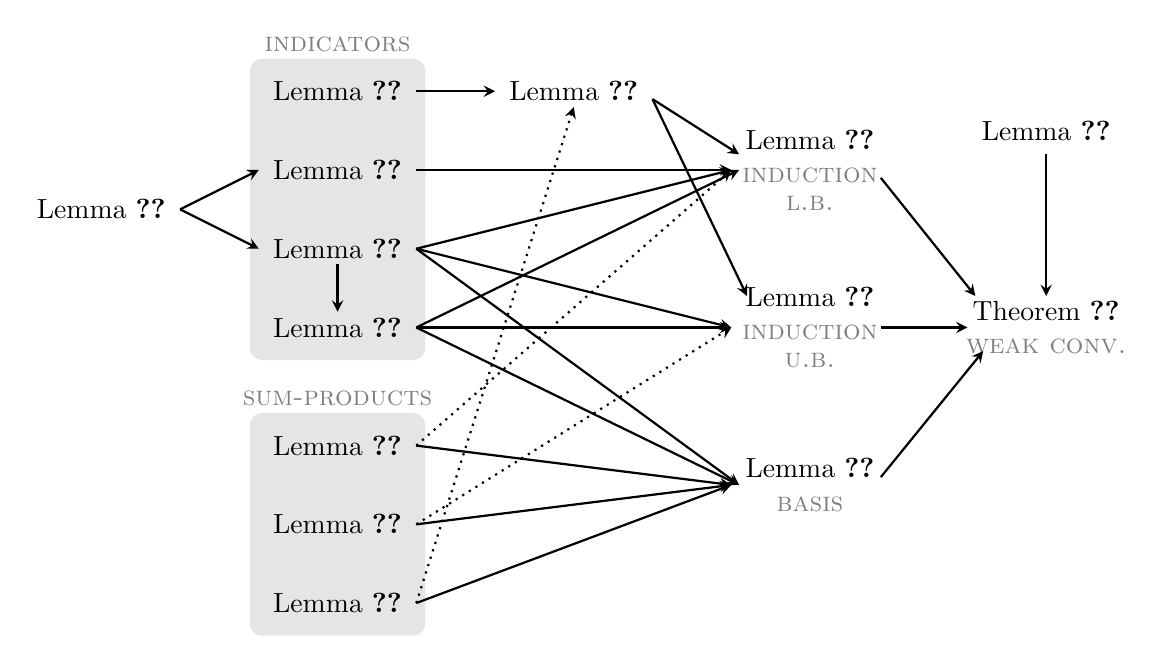
\begin{tikzpicture}[>=stealth, thick]
% boxes
\filldraw[rounded corners, gray!20] (1.9,1.4)--(4.1,1.4)--(4.1,-2.4)--(1.9,-2.4)--cycle;
\node[gray] at (3,1.6) {\textsc{indicators}};
\filldraw[rounded corners, gray!20] (1.9,-3.1)--(4.1,-3.1)--(4.1,-5.9)--(1.9,-5.9)--cycle;
\node[gray] at (3,-2.9) {\textsc{sum-products}};

% nodes column 1
\node at (0,-0.5) {Lemma~\ref{thm:kjjslemma2}};
%nodes column 2 indics
\node at (3,1) {Lemma~\ref{thm:indicators_c2}};
\node at (3,0) {Lemma~\ref{thm:indicators_DN}};
\node at (3,-1) {Lemma~\ref{thm:indicators_cN}};
\node at (3,-2) {Lemma~\ref{thm:indicators_tau}};
% nodes column 2 sumprods
\node at (3,-3.5) {Lemma~\ref{thm:sumprod3}};
\node at (3,-4.5) {Lemma~\ref{thm:sumprod2}};
\node at (3,-5.5) {Lemma~\ref{thm:sumprod1}};
%nodes column 3
\node at (6,1) {Lemma~\ref{thm:induction_sumprodcN}};
% nodes column 4
\node[align=center] at (9,0) {Lemma~\ref{thm:inductionLB}\\[-3pt] 
    \textcolor{gray}{\textsc{induction}} \\[-5pt] \textcolor{gray}{\textsc{l.b.}} };
\node[align=center] at (9,-2) {Lemma~\ref{thm:inductionUB}\\[-3pt] 
    \textcolor{gray}{\textsc{induction}} \\[-5pt] \textcolor{gray}{\textsc{u.b.}} };
\node[align=center] at (9,-4) {Lemma~\ref{thm:basis}\\[-3pt] 
    \textcolor{gray}{\textsc{basis}} };
%nodes column 5
\node at (12,0.5) {Lemma~\ref{thm:maximum_pr}};
\node[align=center] at (12,-2) {Theorem~\ref{thm:weakconv}\\[-3pt] 
    \textcolor{gray}{\textsc{weak conv.}} };

% arrows column 1 to 2
\draw[->] (1,-0.5)--(2,0);
\draw[->] (1,-0.5)--(2,-1);
%arrows column 2 to 2
\draw[->] (3,-1.2)--(3,-1.8);
%arrows column 2 to 3
\draw[->] (4,1)--(5,1);
\draw[->, dotted] (4,-5.5)--(6,0.8);
%arrows column2 indics to 4
\draw[->] (4,-2)--(8.1,0);
\draw[->] (4,-2)--(8,-2);
\draw[->] (4,-2)--(8.1,-4);
\draw[->] (4,-1)--(8,0);
\draw[->] (4,-1)--(8,-2);
\draw[->] (4,-1)--(8.1,-4);
\draw[->] (4,0)--(8,0);
% arrows column 2 sumprods to 4
\draw[->, dotted] (4,-3.5)--(8,0);
\draw[->, dotted] (4,-4.5)--(8,-2);
\draw[->] (4,-3.5)--(8,-4);
\draw[->] (4,-4.5)--(8,-4);
\draw[->] (4,-5.5)--(8,-4);
% arrows column 3 to 4
\draw[->] (7,0.9)--(8.1,0.2);
\draw[->] (7,0.9)--(8.2,-1.6);
%arrows column 4 to 5
\draw[->] (9.9,-0.1)--(11.1,-1.6);
\draw[->] (9.9,-2)--(11,-2);
\draw[->] (9.9,-3.9)--(11.2,-2.3);
% arrows column 5 to 5
\draw[->] (12,0.2)--(12,-1.6);
\end{tikzpicture}
\caption[Structure of weak convergence proof]{Graph showing dependencies between the lemmata used to prove weak convergence. Dotted arrows indicate dependence via a slight modification of the preceding lemma. \seb{Add FDD convergence theorem as another precedent of weak convergence theorem.}}
\end{figure}

%\chapter{Discussion}

\epigraph{
I never see what has been done; I only see what remains to be done.
}
{\textsc{Marie Curie}}

We have provided a simple sufficient condition for genealogies of SMC particle systems to converge to Kingman's $n$-coalescent in the large population limit. 
This result complements existing work not only in the SMC literature but also in mathematical population genetics, where it shows that non-neutral population models can produce $n$-coalescents in the limit, under conditions analogous to those required for neutral models.

We have demonstrated that our convergence condition is verifiable in a range of settings, including SMC algorithms using many of the most popular resampling schemes. 
Convergence to a coalescent limit requires a random rescaling of time, governed by the function $\tau_N$, which can be viewed as encoding the genealogical behaviour of each algorithm.
Information about this time-sclae function could therefore be used to directly compare the ancestral degeneracy of different algorithms, solve tuning problems, or quantify asymptotic behaviour of SMC estimators.

I believe that the main limitation of the work, therefore, is our lack of information about $\tau_N$. An interesting topic of future research would be to characterise this function a priori, say for a particular tractable class of models.
From there it would be possible to find the limiting distributions of many statistics of interest, such as the time to full coalescence or the probability of maintaining a certain number of distinct lineages over a given time window. It would also allow a comaprison between the genealogies arising from different resampling schemes.

I will finish by describing three more open questions raised by the current work, which I believe to be interesting avenues for future research. These problems are, in my opinion, less critical than that of characterising the time-scale function, but probably easier to tackle. 
I hope that a future researcher may find these to be interesting diversions.

In neutral models, the neutral version of our main condition has been shown to be necessary and sufficient for convergence to the $n$-coalescent. This raises the question: are our conditions necessary as well as sufficient, or else what alterations are needed to render them necessary and sufficient?

We have shown that our convergence theorems apply to a range of SMC algorithms, encompassing most of the resampling schemes that are routinely used by practitioners. A notable exception is residual resampling with multinomial residuals, which, although not generally recommended by theorists, is frequently used in practice.
There is no reason to believe that the convergence results should not apply in this case: we have seen that by various metrics residual-multinomial resampling lies between multinomial and, say, residual-systematic resampling, both of which have been shown to satisfy the conditions of the theorems.
However, we have not yet succeeded in proving a corollary for residual-multinomial resampling.

Adaptive resampling is routinely used to improve the performance of SMC, and it clearly mitigates the problem of ancestral degeneracy. It is not immediately clear, however, what exactly is the effect of adaptive resampling on the resulting genealogies. At first sight one might imagine that it simply slows the coalescent time scale by some factor determined by how often resampling occurs, but this is not the whole picture. Adaptive resampling must also affect the distribution of the weights that are input to the resampling procedure, because when resampling is triggered the weights necessarily have variance above a certain threshold.
The resulting genealogies may be expected to exhibit long waiting times between coalescence events, and bigger coalescences when they do occur, perhaps even to the point of retaining large or simultaneous mergers in the limit.



\backmatter

%%% A list of acronyms must be placed either here or after the abstract, and its location indicated in the ToC.

%%% The bibliography/references will go here.
\printbibliography

\end{document}